%% Copernicus Publications Manuscript Preparation Template for LaTeX Submissions
%% ---------------------------------
%% This template should be used for copernicus.cls
%% The class file and some style files are bundled in the Copernicus Latex Package, which can be downloaded from the different journal webpages.
%% For further assistance please contact Copernicus Publications at: production@copernicus.org
%% https://publications.copernicus.org/for_authors/manuscript_preparation.html


%% Please use the following documentclass and journal abbreviations for preprints and final revised papers.

%% 2-column papers and preprints
\documentclass[journal abbreviation, manuscript]{copernicus}



%% Journal abbreviations (please use the same for preprints and final revised papers)


% Advances in Geosciences (adgeo)
% Advances in Radio Science (ars)
% Advances in Science and Research (asr)
% Advances in Statistical Climatology, Meteorology and Oceanography (ascmo)
% Aerosol Research (ar)
% Annales Geophysicae (angeo)
% Archives Animal Breeding (aab)
% Atmospheric Chemistry and Physics (acp)
% Atmospheric Measurement Techniques (amt)
% Biogeosciences (bg)
% Climate of the Past (cp)
% DEUQUA Special Publications (deuquasp)
% Earth Surface Dynamics (esurf)
% Earth System Dynamics (esd)
% Earth System Science Data (essd)
% E&G Quaternary Science Journal (egqsj)
% EGUsphere (egusphere) | This is only for EGUsphere preprints submitted without relation to an EGU journal.
% Earth Observation (eo)
% European Journal of Mineralogy (ejm)
% Geochronology (gchron)
% Geographica Helvetica (gh)
% Geoscience Communication (gc)
% Geoscientific Instrumentation, Methods and Data Systems (gi)
% Geoscientific Model Development (gmd)
% History of Geo- and Space Sciences (hgss)
% Hydrology and Earth System Sciences (hess)
% Journal of Bone and Joint Infection (jbji)
% Journal of Environmentally Compatible Air Transport System (jecats)
% Journal of Micropalaeontology (jm)
% Journal of Sensors and Sensor Systems (jsss)
% Magnetic Resonance (mr)
% Mechanical Sciences (ms)
% Natural Hazards and Earth System Sciences (nhess)
% Nonlinear Processes in Geophysics (npg)
% Ocean Science (os)
% Polarforschung - Journal of the German Society for Polar Research (polf)
% Proceedings of the International Association of Hydrological Sciences (piahs)
% Proceedings of the International Ocean Drilling Programme (piodp)
% Safety of Nuclear Waste Disposal (sand)
% Scientific Drilling (sd)
% SOIL (soil)
% Solid Earth (se)
% State of the Planet (sp)
% The Cryosphere (tc)
% Weather and Climate Dynamics (wcd)
% Web Ecology (we)
% Wind Energy Science (wes)


%% \usepackage commands included in the copernicus.cls:
\usepackage{booktabs}
\usepackage{tabularx}
\usepackage{cancel}
\usepackage{multirow}
\usepackage{supertabular}
\usepackage{algorithmic}
\usepackage{algorithm}
\usepackage{amsthm}
\usepackage{float}
\usepackage{subfig}
\usepackage{rotating}


\runningtitle{Latent spatial structure in landslide susceptibility}
\runningauthor{E. Aristizábal et al.}

\begin{document}

\title{The dominant role of latent spatial structure in landslide susceptibility}


% \Author[affil]{given_name}{surname}

\Author[1,3][evaristizabalg@unal.edu.co]{Edier}{Aristizábal} %% correspondence author
\Author[2]{Luigi}{Lombardo}
\Author[3]{Oliver}{Korup}

\affil[1]{Departamento de Geociencias y Medio Ambiente, Universidad Nacional de Colombia, Medellín, Colombia}
\affil[2]{Faculty of Geo-Information Science and Earth Observation (ITC), University of Twente, Enschede, Netherlands}
\affil[3]{Institute of Environmental Science and Geography, University of Potsdam, Potsdam, Germany}

\received{}
\pubdiscuss{} %% only important for two-stage journals
\revised{}
\accepted{}
\published{}

\firstpage{1}

\maketitle

\begin{abstract}
Landslide susceptibility mapping is essential for risk management and mitigation. 
Traditional multivariate models have achieved high nominal accuracy in predicting landslide occurrence, but the underlying methods rarely account for spatial dependence in the input data. 
We test how spatial Hierarchical Generalized Linear Models (HGLMs) and spatial autoregressive models might enhance both accuracy and reliability of landslide susceptibility. 
We estimate the frequency of landslides in a catchment, drawing on a catalogue of 10,837 landslides and several predictors (e.g., rainfall, elevation, slope) in the northern Colombian Andes. 
Our HGLMs integrate the effects of spatial dependency and heterogeneity through Markov Random Field (MRF) models, i.e. Intrinsic Conditional Autoregressive (ICAR), Besag-York-Mollié (BYM), and Leroux models. 
Our results show that landslide frequency is significantly influenced by spatially-dependent unobserved factors, likely representing contiguous geological formations or shared soil properties, which we therefore incorporate as latent variables. 
Even after accounting for known covariates, the HGLMs
capture spatial dependencies that non-spatial models fail to address. Incorporating spatial structure in
the data improves model performance, judging from model selection metrics such as the Deviance Information Criterion (DIC) or the Watanabe–Akaike Information Criterion (WAIC). By accounting for latent
spatial effects, spatial HGLMs produce smoother and more reliable susceptibility maps. This approach
overcomes a key limitation of traditional models: the underestimation of landslide frequency in high-
density areas where unobserved, spatially-structured factors are most influential. Our findings highlight
the importance of integrating spatial dependence and heterogeneity in landslide susceptibility models to
achieve enhanced predictive performance and reliability.
\end{abstract}

\introduction 
The primary objective of landslide susceptibility studies is to map how likely a given terrain portion is to slope failure, based on some known spatial distribution of landslides \citep{fell2008guidelines, corominas2014recommendations, soeters1996slope}. Statistical studies that tackle this task rely on a set of predictors (also termed covariates, or independent variables) that may reflect whether a landslide is likely at a given location \citep{reichenbach2018review, steger2019statistical}. These predictors are essentially spatial data that can be cross-sectional, represented by discrete terrain mapping units (TMUs) at a given time slice \citep{elhorst2014spatial}, or panel data that encompass values from TMUs over several time slices.

TMUs are known as areal or lattice data in spatial statistics, and are regular or irregular homogeneous subdivisions of the terrain used to discretize and aggregate data relevant to landslide susceptibility \citep{carrara1995gis, erener2012landslide}. Pixels or grid cells are the most common TMUs, straightforward to define, and easy to use in computation \citep{ba2018comparison}. Irregular TMUs, such as slope units \citep{tanyas2019global, alvioli2016automatic}, unique conditions \citep{clerici2002procedure}, or catchments \citep{von2013rainfall, shou2020evaluation}, are physically more meaningful, but require some pre-processing \citep{caleca2025pan}.

Although recent research has highlighted spatial effects in landslide susceptibility \citep{lombardo2019geostatistical}, few studies have explicitly considered or evaluated these effects. In this context, spatial effects comprise two main components at two distinct levels: spatial heterogeneity, which reflects large-scale variations between regions that reflect differences in environmental, geological, or geographical conditions; and spatial dependence, where processes in one location are influenced by those in its immediate neighborhood. For example, \citet{samia2019dynamic} proposed the concept of landslide path dependence, arguing that once a landslide occurs, it can serve as an attractor for future landslides, making subsequent events more likely to occur within or near its vicinity. \citet{lombardo2019geostatistical} identified significant spatial structures in event-based landslide analyses, even when triggers like precipitation or seismic activity were excluded from the covariates.

A persistent challenge is that landslide occurrence cannot be fully explained by predictors alone \citep{di2023estimation}. This unresolved variance, often visible as spatial patterns in model residuals, may stem from either missing covariates or from inherent spatial processes that are not captured by the predictors. Spatial landslide patterns may not simply mimic those of the predictors \citep{lombardo2020space}, but also include interactions between neighboring TMUs. Most currently used susceptibility models are not designed to account for such spatial structure and interactions between neighboring units \citep{fang2023space}. Thus, spatial effects often remain in model residuals, while violating the key assumption of identical and independence distributions (i.i.d.) in likelihood-based models \citep{wagner2013rethinking}. This oversight artificially lowers p-values and standard errors of parameter estimates, inflating the statistical relevance of predictors \citep{lee2021network, lombardo2020space}. Hence, these models may become overconfident in their predictions. Beyond representing unaccounted for variability, any residual spatial effects may contain valuable information about physical drivers of landslide occurrence. Hence, there is a need for comprehensive modeling approaches that capture these spatial effects. This residual spatial structure often acts as a proxy for unobserved but spatially correlated factors, such as local geological characteristics, soil property variations, or fine-scale anthropogenic effects, which are not captured by the regional-scale covariates. Therefore, failing to model this spatial structure is not just a statistical oversight; it is a failure to account for the physical, spatially-organized predictors that govern landslide initiation. This can lead to maps that misidentify susceptibility by ignoring this crucial geological context.

Recent research has advanced hierarchical spatial modeling approaches that account for spatial effects \citep{dong2015multilevel, morris2019bayesian, lawson2018bayesian}. For example, Hierarchical Spatial Autoregressive (HSA) models have been successfully applied in fields such as disease mapping \citep{vranckx2019comparison}, the modeling of social well-being \citep{pierewan2014spatial}, and land-market analysis \citep{dong2015multilevel}. However, to the best of our knowledge, HSA models have not yet been implemented in landslide susceptibility mapping. More generally, spatial modeling approaches are still hardly used in landslide susceptibility assessment. One exception is the work by \citet{lombardo2018point, lombardo2019geostatistical, lombardo2020space}. By using a continuous-space point process with a latent spatial effect, they demonstrated that landslide patterns are not simply a reflection of the predictors' spatial distribution. Their key finding was that significant spatial dependencies remain even when triggers like precipitation or seismic shaking are included in the model, pointing to the importance of underlying, unmeasured processes.

HSAs are usually implemented within a Bayesian framework that requires numerical approximation methods such as Markov Chain Monte Carlo (MCMC). A newer, faster, and computationally less expensive method Integrated Nested Laplace Approximation (INLA) has been proposed by \citet{rue2005gaussian} as a viable alternative.

Therefore, the primary objective of this study is to test and compare several spatial HGLMs for landslide susceptibility mapping in the northern Colombian Andes. We first establish a non-spatial baseline model and then progressively incorporate spatial effects, including random intercepts for regional heterogeneity and different conditional autoregressive structures (ICAR, BYM, and Leroux) for local spatial dependence. By systematically comparing these models, we aim to quantify the improvement in predictive performance and demonstrate the critical importance of accounting for spatial structure to produce more accurate and reliable susceptibility assessments that better reflect the underlying physical processes and geological controls.


\section{Generalised Linear Models (GLM)}\label{sec2}

Generalized Linear Model (GLM)-based methods are popular to model landslide susceptibility because they are easy to interpret and extend \citep{reichenbach2018review, corominas2014recommendations, guzzetti1999landslide}. They encompass a broad class of models where the response variable ($y$) is assumed to follow an exponential family distribution \citep{coxe2013generalized, hastie2017generalized}, such as Gaussian, Poisson, Binomial, or Gamma. The expected value of the response ($E(y) = \mu$) is modeled by a linear predictor ($\eta$) through a link function ($g(\mu) = \eta$) that assumes additive effects (or weights) of covariates. GLMs can accommodate both continuous and discrete predictors \citep{camilo2017handling, goetz2011integrating}.

Logistic regression has been a long-standing GLM method for modeling landslide susceptibility \citep{david2000applied, ayalew2005application}, and uses a logit link function to map the linear combination of predictors $\sum_{j=1}^k \beta_j x_{ij}$ to values of the unit interval, which represents a probability scale of success under a Bernoulli likelihood \citep{david2000applied}, where $x_{ij}$ is the value of the $j$-th predictor for the $i$-th observation, and $\beta_{j}$ is its corresponding regression coefficient. However, the application of logistic regression to data aggregated into TMUs presents a fundamental limitation. The model requires a dichotomous (presence/absence) response variable, which necessitates the binarization of what is inherently count data. This process results in a loss of information regarding event density, which can confound the true relationship between conditioning factors and landslide frequency, an effect that is also scale-dependent \citep{lombardo2018point}. Poisson regression is another GLM member that models count data $Y$, and allows for aggregating landslide counts and probabilities across TMUs \citep{tay2014landslide, opitz2022high}. The Poisson distribution has a single parameter, $\lambda$, which is both the mean and variance.

\begin{equation}
Y \sim Poisson(\lambda)
\end{equation}
\begin{equation}
E(Y) = \lambda
\end{equation}
\begin{equation}
var(Y) = \lambda
\end{equation}

Poisson regression uses an exponential link function to estimate $\lambda$:

\begin{equation}
\lambda_i = \exp(\eta_i)
\end{equation}
\begin{equation}
\eta_i = \alpha + \sum_{j=1}^k \beta_j x_{ij} + \log(A_i)
\end{equation}

\subsection{Spatial hierarchical structure}\label{subsec21}

Spatial effects in a GLM can occur at two distinct levels. At the higher level, spatial heterogeneity is often hierarchical or contextual, capturing a top-down or vertical effect in the data structure, where the properties of an individual TMU (like a catchment) are partly determined by the broader characteristics of the group it belongs to (like a basin) \citep{corrado2011multilevel}. At the lower level, spatial dependency reflects the continuity of physical processes like erosion, hydrology, or slope instability \citep{cellmer2019application}.

GLMs can be cast in hierarchical structures to account for spatial heterogeneity in predictors \citep{lee1996hierarchical, lee2017data}, such that regression coefficients vary across spatial domains \citep{atkinson1998generalized, ma2021bayesian, dalthorp2004generalized}. Coefficients in hierarchical models are separated into fixed effects, associated with lower-level units (e.g., TMUs) and random effects, which represent variability at the upper level (e.g., basins or regions). Fixed effects refer to the regression coefficients that represent the central tendency of the model \citep{torres2007panel}, whereas random effects are parameters that may influence the target variable beyond the primary focus of the model \citep{firebaugh2013fixed}. In terms of the Poisson regression, both can be cast as:

\begin{equation}
\eta_i = \underbrace{\alpha + \sum_{j=1}^k \beta_j x_{ij} + \log(A_i)}_{\text{fixed effects}} + \underbrace{\sum_{l=1}^r \gamma_l z_{il} + \varepsilon_i}_{\text{random effects}}
\end{equation}

The random effects include $r$ components, where $z_{il}$ is the value of the $l$-th random effect component for the $i$-th observation with coefficient $\gamma_{l}$. Finally, $\varepsilon_i$ represents the spatially structured random effects, and $\log(A_i)$ is the offset term to account for the area of the TMU.

Although HGLMs are frequently applied to spatial data, they are not full spatial models \citep{dong2015multilevel}, and limited in their assumption that covariate effects at lower levels are independent of each other, thereby neglecting spatial dependence \citep{raudenbush2002hierarchical, goldstein2011multilevel}. While HGLMs naturally capture spatial effects within higher levels and provide a flexible framework for modeling the spatial heterogeneity of predictors, these models fail to capture neighborhood structures and spatial dependency \citep{dong2015multilevel, osland2016accounting, rabe2008multilevel}.

\subsection{Spatial Autoregressive models}\label{subsec22}

The latent spatial effect at the lower level represents the unexplained, but spatially structured (horizontal or proximity-based), component of the data that remains after accounting for the predictor effects \citep{austin2013covariate, aigner1984latent}. Spatial statistics offer various approaches to incorporate spatial dependence at a lower level. For discrete data, such as TMUs, auto-regressive models are often recommended, where the spatial structure is represented by a neighborhood connectivity matrix \citep{rodrigues2012bayesian}, and determines whether TMUs are neighbors based on metrics such as contiguity, distance, or nearest neighbors \citep{moraga2023spatial}.

The two most common auto-regressive models for discrete data are the Simultaneously Autoregressive (SAR) and Conditionally Autoregressive (CAR) models \citep{jaya2021spatial}. The primary distinction between them is the scope of the spatial dependence. SAR models treat this dependence as a global process, where the spatial effect is incorporated as a new term reflecting the influence of all other locations, typically in the response variable or the error term \citep{hooten2014simultaneous, anselin1988spatial}. In contrast, CAR models define spatial dependence as a local process and are a type of Markov Random Field (MRF) \citep{earnest2007evaluating, besag1991bayesian}. A spatial process is considered to have the Markov property if the state of a parameter depends only on its immediately adjacent neighbors, making it conditionally independent of all other locations \citep{clifford1990markov, rue2005gaussian}. The most common form of MRF represents this first-order neighborhood connectivity in terms of contiguity, where TMUs sharing a boundary are considered neighbors.

The Markov assumption of CAR models is physically well-suited for landslides, as the geotechnical and geomorphological properties (e.g., soil depth, weathering grade, rock fractures) of one catchment are most likely to be similar to its immediate neighbors rather than to catchments far away.

Several models have been proposed within a class of CAR structures, including intrinsic and convolution models \citep{besag1991bayesian}, as well as alternatives such as Leroux CAR \citep{leroux2000estimation}. The intrinsic CAR (ICAR) model is the simplest CAR structure, assuming a spatially autoregressive random effect to address associations among neighboring regions \citep{besag1991bayesian}. The conditional expectation equals the mean of the random effects in neighboring TMUs, while the conditional variance is inversely proportional to the number of its neighbors. This model represents strong spatial correlation structures and may be unsuitable if the predictors are weakly correlated.

\citet{besag1991bayesian} proposed the convolution model, or Besag-York-Molli\'{e} (BYM) model, which combines two latent random effects, i.e. an ICAR latent effect ($\rho$) and an i.i.d. Gaussian latent effect ($\sigma$). However, the two separate random effects components cannot be individually identified, and only their sum is identifiable.

\citet{leroux2000estimation} proposed using a single random effect instead, including a parameter ($\rho$) to measure the level of spatial correlation among terrain mapping units, taking values on the unit interval. This model is a variation of the BYM and ICAR models. Like the ICAR model, it has one spatial random-effect parameter for each TMU. However, the conditional distribution incorporates characteristics of both structured and unstructured spatial random effects (from the BYM model) into a single parameter ($\rho$). The Leroux model generalizes the ICAR model and the independent model (i.e., a model without any structured spatial random effect). When $\rho = 1$, the ICAR model is recovered; when $\rho = 0$, the independent model is recovered instead. Thus, the Leroux model seeks to balance these two models by estimating the value of $\rho$.

The choice between these models has physical implications. An ICAR model assumes a very strong, smooth spatial process, suggesting that unobserved factors (like a large, contiguous geological formation) are dominant. The BYM and Leroux models are more flexible, allowing the data to decide how much of the unexplained variance is due to this structured spatial process (the 'geology') and how much is just unstructured random noise (local variability unique to that specific catchment and not shared).

\subsection{Bayesian inference framework}\label{subsec23}

Bayesian methods are well-suited for handling spatial data because they are informed by prior knowledge, handle uncertainty in a probabilistic manner, and can model complex spatial dependencies.

The fundamental concept of the Bayesian approach is to use probability to quantify uncertainty in all unknown aspects of a statistical model \citep{johnson2022bayes}. The uncertainty about the model parameters, given the current state of knowledge and without observing any new data, is described by a prior distribution. The inferential process combines the prior and the current data model (i.e. a likelihood function of the model parameters) to derive a posterior distribution, which is typically the objective of the inference \citep{congdon2014applied}.

Fitting a Bayesian model involves computing the joint posterior distribution of the latent field $x$ and the hyperparameters $\theta$, denoted as $p(\theta, x|y)$, using Bayes' rule:

\begin{equation}
p(\theta,x | y) = \frac{p(y | x,\theta) p(x | \theta) p(\theta)}{p(y)}
\end{equation}

In the context of our landslide susceptibility model, these terms have specific physical interpretations. The latent field ($x$) represents all the unobserved spatial processes that influence where landslides occur. It is the combination of the known effects of your predictors (constructed from fixed effects) and the spatial random effects, which account for unmeasured but spatially structured factors, such as those modeled using a Conditional Autoregressive (CAR) prior.

The hyperparameters ($\theta$), in turn, are the parameters of the prior distributions that control the overall behaviour of this latent field. For instance, they determine the variance of the spatial random effects (i.e., the degree of smoothness in the final susceptibility map) or the strength of the spatial correlation, $\rho$, in the Leroux model (i.e., how much a catchment's susceptibility is influenced by its neighbors).

The term $p(x|\theta)$ represents the prior distribution for the latent field, which mathematically formalizes our assumptions about its structure. A key component of our latent field is the vector of spatial random effects, denoted as $u$. We assume these spatial effects follow a Gaussian Markov Random Field (GMRF) structure, where the neighborhood relationships are defined by a precision matrix $Q(\theta)$. Specifically, the prior for the vector of spatial random effects $u$ is defined as a multivariate normal distribution:

\begin{equation}
u \sim N(0,Q^{-1}(\theta))
\end{equation}

Depending on the likelihood and the prior distribution, computing $p(\theta, x|y)$ can be challenging \citep{gallagher2009markov} or impossible analytically. Several computational sampling approaches, such as Monte Carlo methods, have been proposed to estimate $\pi(\theta, x|y)$. Markov Chain Monte Carlo (MCMC) provides simulations from the ensemble of model parameters \citep{brooks1998markov} to approximate the joint posterior distribution using random sampling. However, MCMC may require many simulations for valid inference, and "burn-in" simulations must be completed to obtain the posterior distribution accurately \citep{jones2022markov}.

Some applications require only marginal inference on some parameters $p(\theta|y)$, and the latent effects are integrated out to obtain the marginal posterior distribution for the hyperparameters. For such cases, \citet{rue2009approximate} proposed the integrated nested Laplace approximation (INLA), which yields univariate distributions that are computationally faster to estimate by numerical integration techniques \citep{gomez2018markov}.

\section{Data and methods}\label{sec3}

To achieve these objectives, we test a HSA model with a Poisson distribution for estimating landslide susceptibility, which we define as the expected number of landslides per catchment in the Colombian Andes. Our model employs a two-level hierarchical structure defined by hydrological scales: the three primary drainage basins (Atrato, Cauca, and Magdalena) serve as the upper level to capture regional heterogeneity (Fig. 1), such as distinct tectonic domains, major lithological groups, or large-scale climatic zones. While the 526 smaller catchments nested within them act as the lower-level Terrain Mapping Units (TMUs), where we model local, proximity-based processes. This is the scale at which factors like rock-mass strength, hillslope-scale hydrology, and shared soil properties create spatial clusters of instability. To account for spatial dependency at the lower level, we test several conditional autoregressive structures.

The study area in the northern Colombian Andes is a tectonically active, mountainous region characterized by steep topography, deep weathering profiles, and intense seasonal rainfall. Consequently, the landscape is dominated by frequent, rainfall-induced slope failures. Our landslide inventory is predominantly composed of shallow translational soil slides and debris flows, which typically mobilize residual soils and saprolite on hillslopes steeper than 25$^{\circ}$. We compiled this inventory of 10,837 that occurred between 1970 and 2023 (Fig. 1) from manual mapping based on true-color optical images from Google Earth Pro (provided by Maxar/Airbus Technologies and Landsat/Copernicus), at a nominal resolution of $<$1 m.

\begin{figure*}[t]
\centering
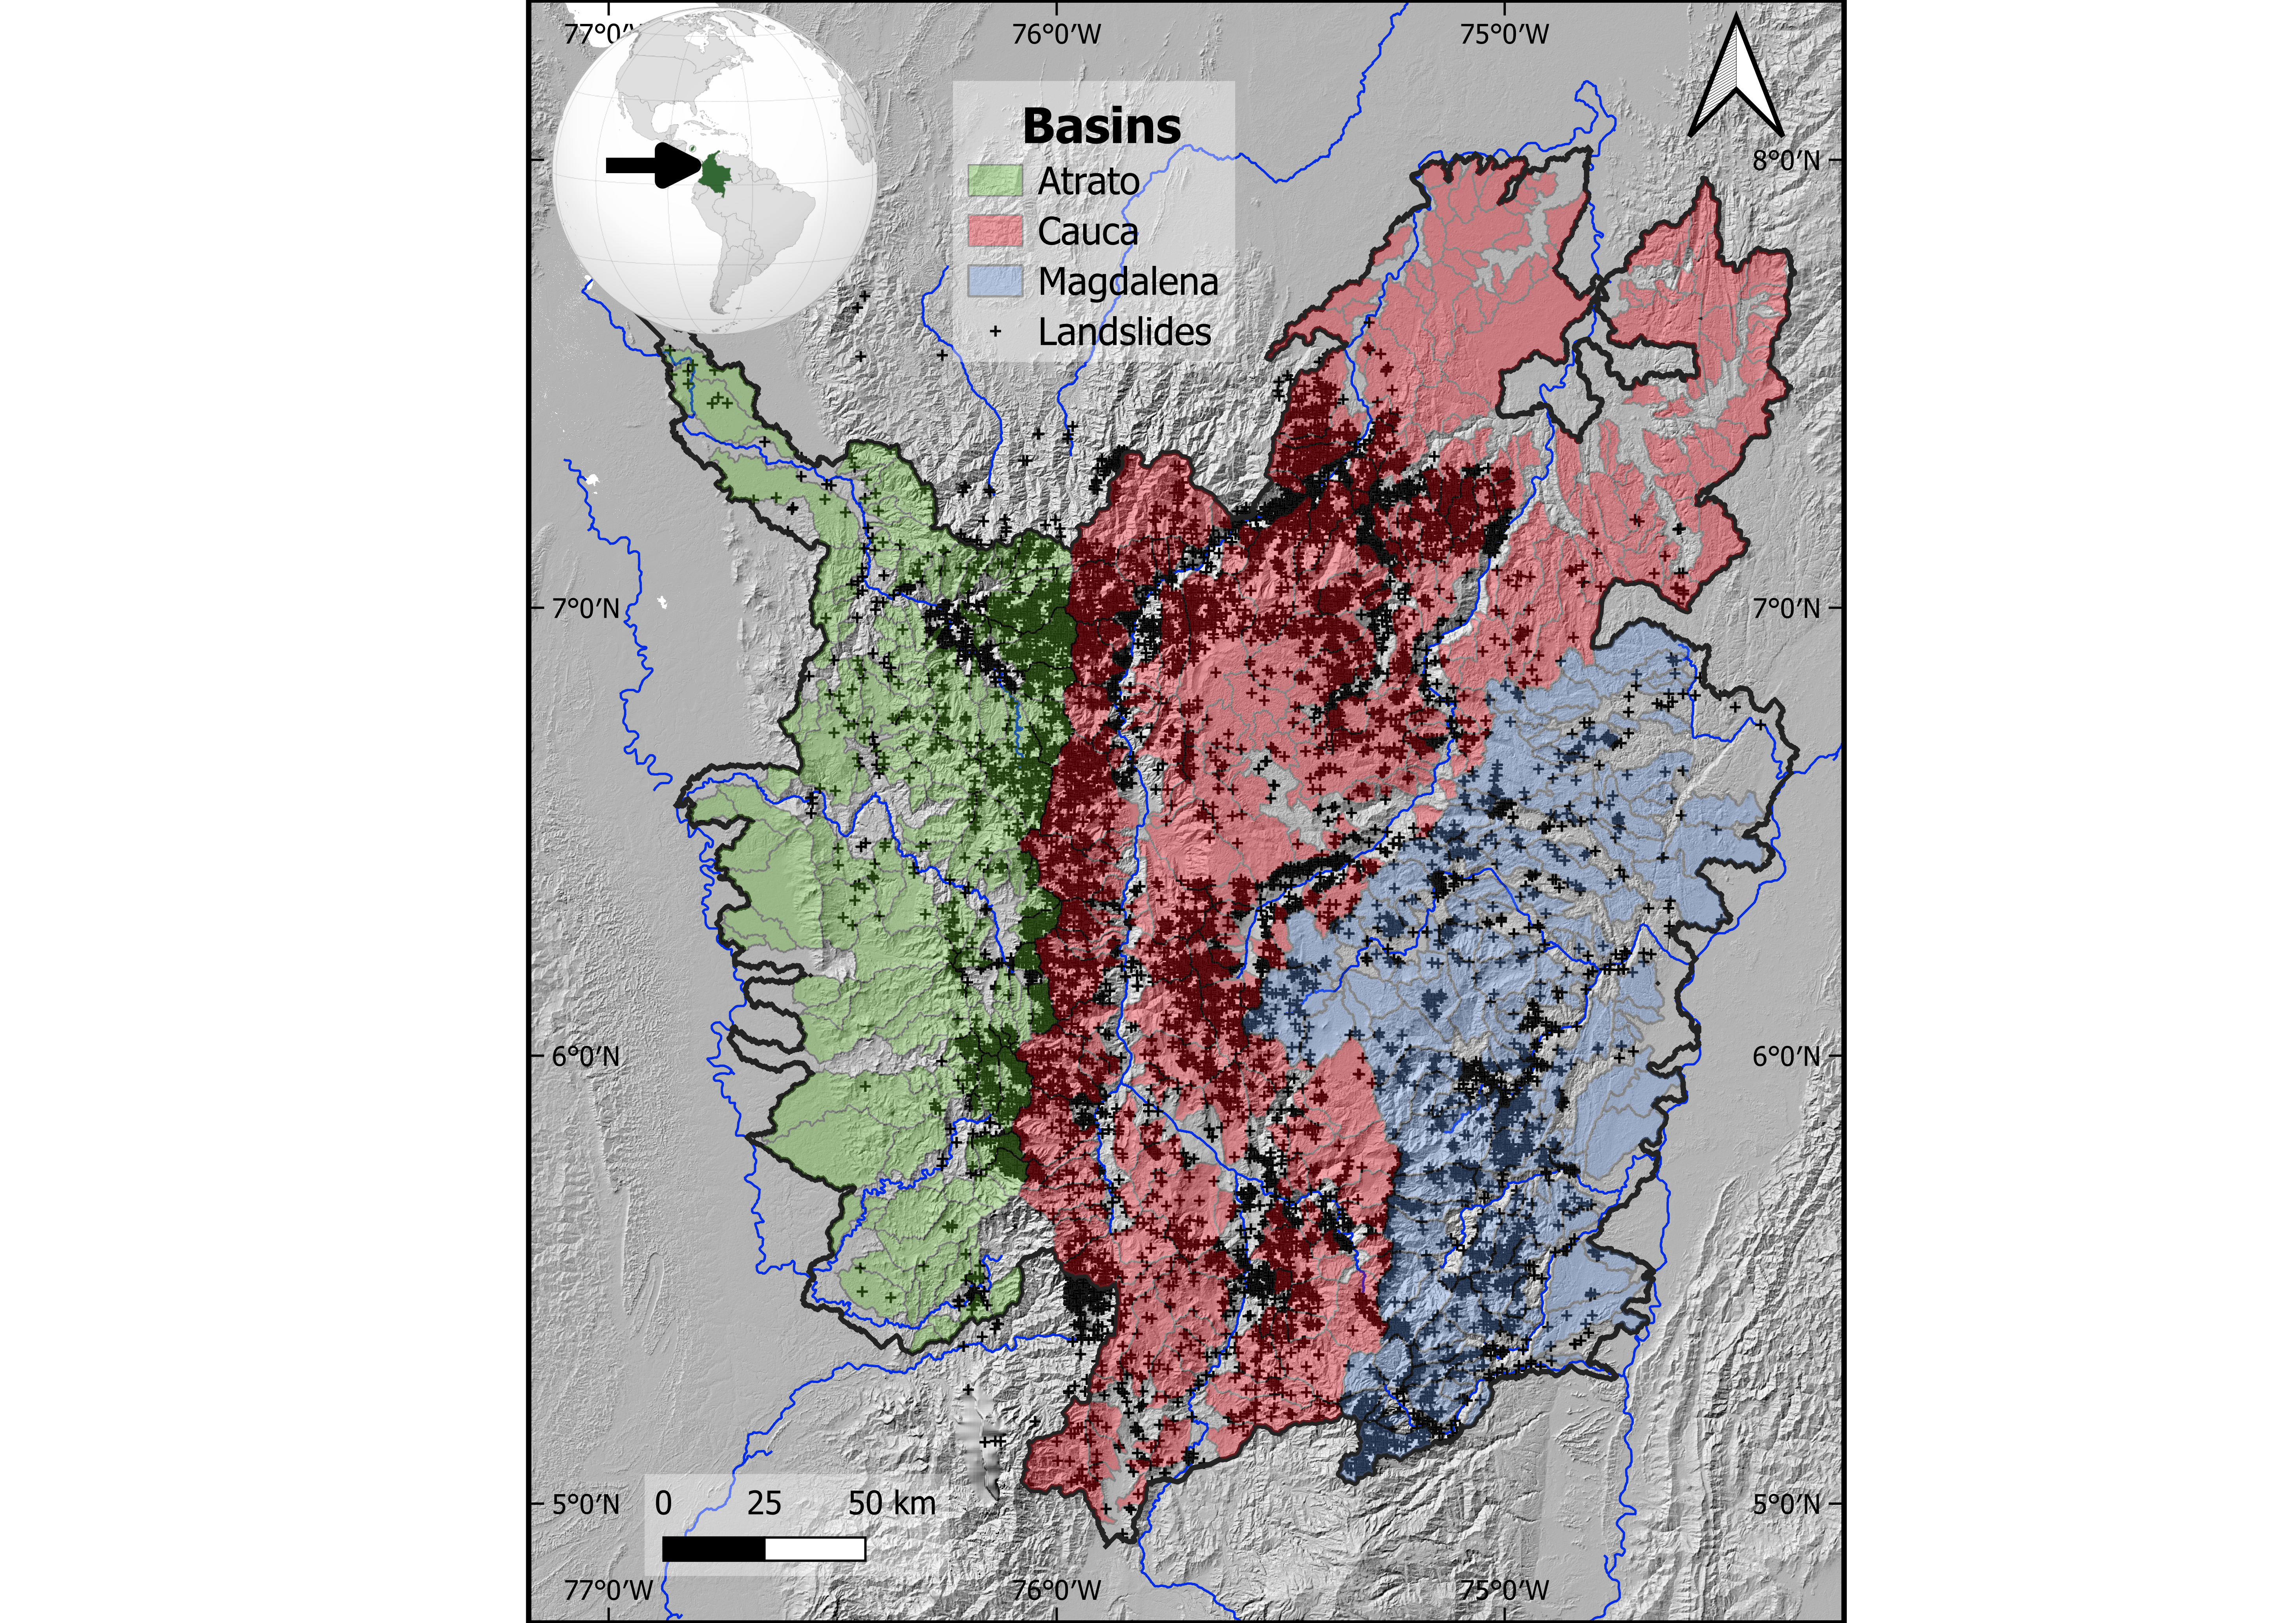
\includegraphics[width=0.7\textwidth]{Fig1A.png}
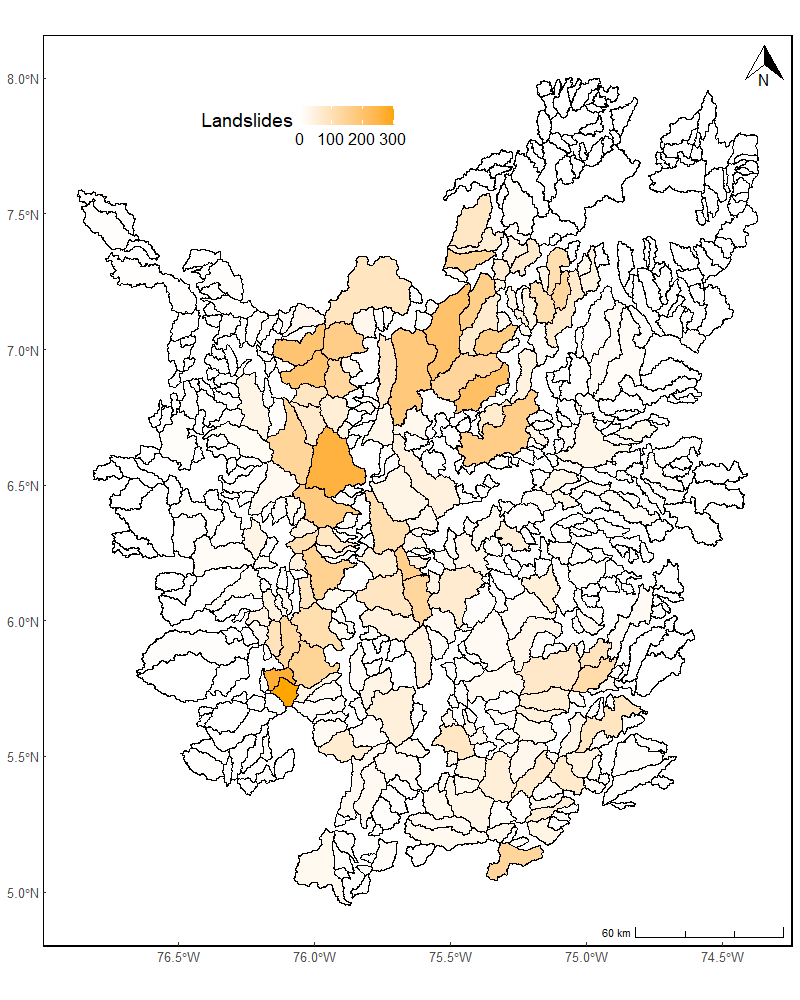
\includegraphics[width=0.4\textwidth]{Fig1B.png}
\caption{Landslide occurrences. (A) Study area in the northern Colombian Andes with the three main basins. (B) Inventory of 10,837 landslides mapped using Google Earth Pro (Imagery © 1970-2023 Google, Maxar/Airbus Technologies \& Landsat/Copernicus)}
\label{Fig1}
\end{figure*}

Aided by correlation matrix analysis and Principal Component Analysis (PCA), we selected three predictors, i.e. the number of days with rainfall totals $>$20 mm ($R_d$); mean elevation ($H$); and mean slope ($S$). These predictors were selected for their direct physical relevance to landslide initiation. $S$ is a primary factor, as steeper terrain increases the shear stress on soils. $R_d$ acts as a proxy for the frequency of triggering events; intense rainfall increases pore-water pressure within the soil. Finally, $H$ often serves as an effective proxy for a combination of factors, including orographic effects on precipitation, variations in geological materials and weathering, and changes in land cover, all of which strongly influence slope stability. We derived the terrain parameters from the digital elevation model (DEM) of the Advanced Land Observing Satellite-Phased Array-Type L-Band Synthetic Aperture Radar (ALOS-PALSAR) at a resolution of 12.5 m \citep{logan2014radiometrically}. We computed $R_d$ from 1981 to 2023 with Google Earth Engine (GEE) using the Climate Hazard Group InfraRed Precipitation with Station Data (CHIRPS) \citep{funk2015climate} version 2.0 at a 5-km resolution.

The spatial structure at the lower level was represented employing the Queen adjacency rule \citep{moraga2023spatial}, where TMUs are considered neighbors if they share at least one border. The derived spatial contiguity weight and covariance matrices are shown in Figure 2.

\begin{figure}[h]
\centering
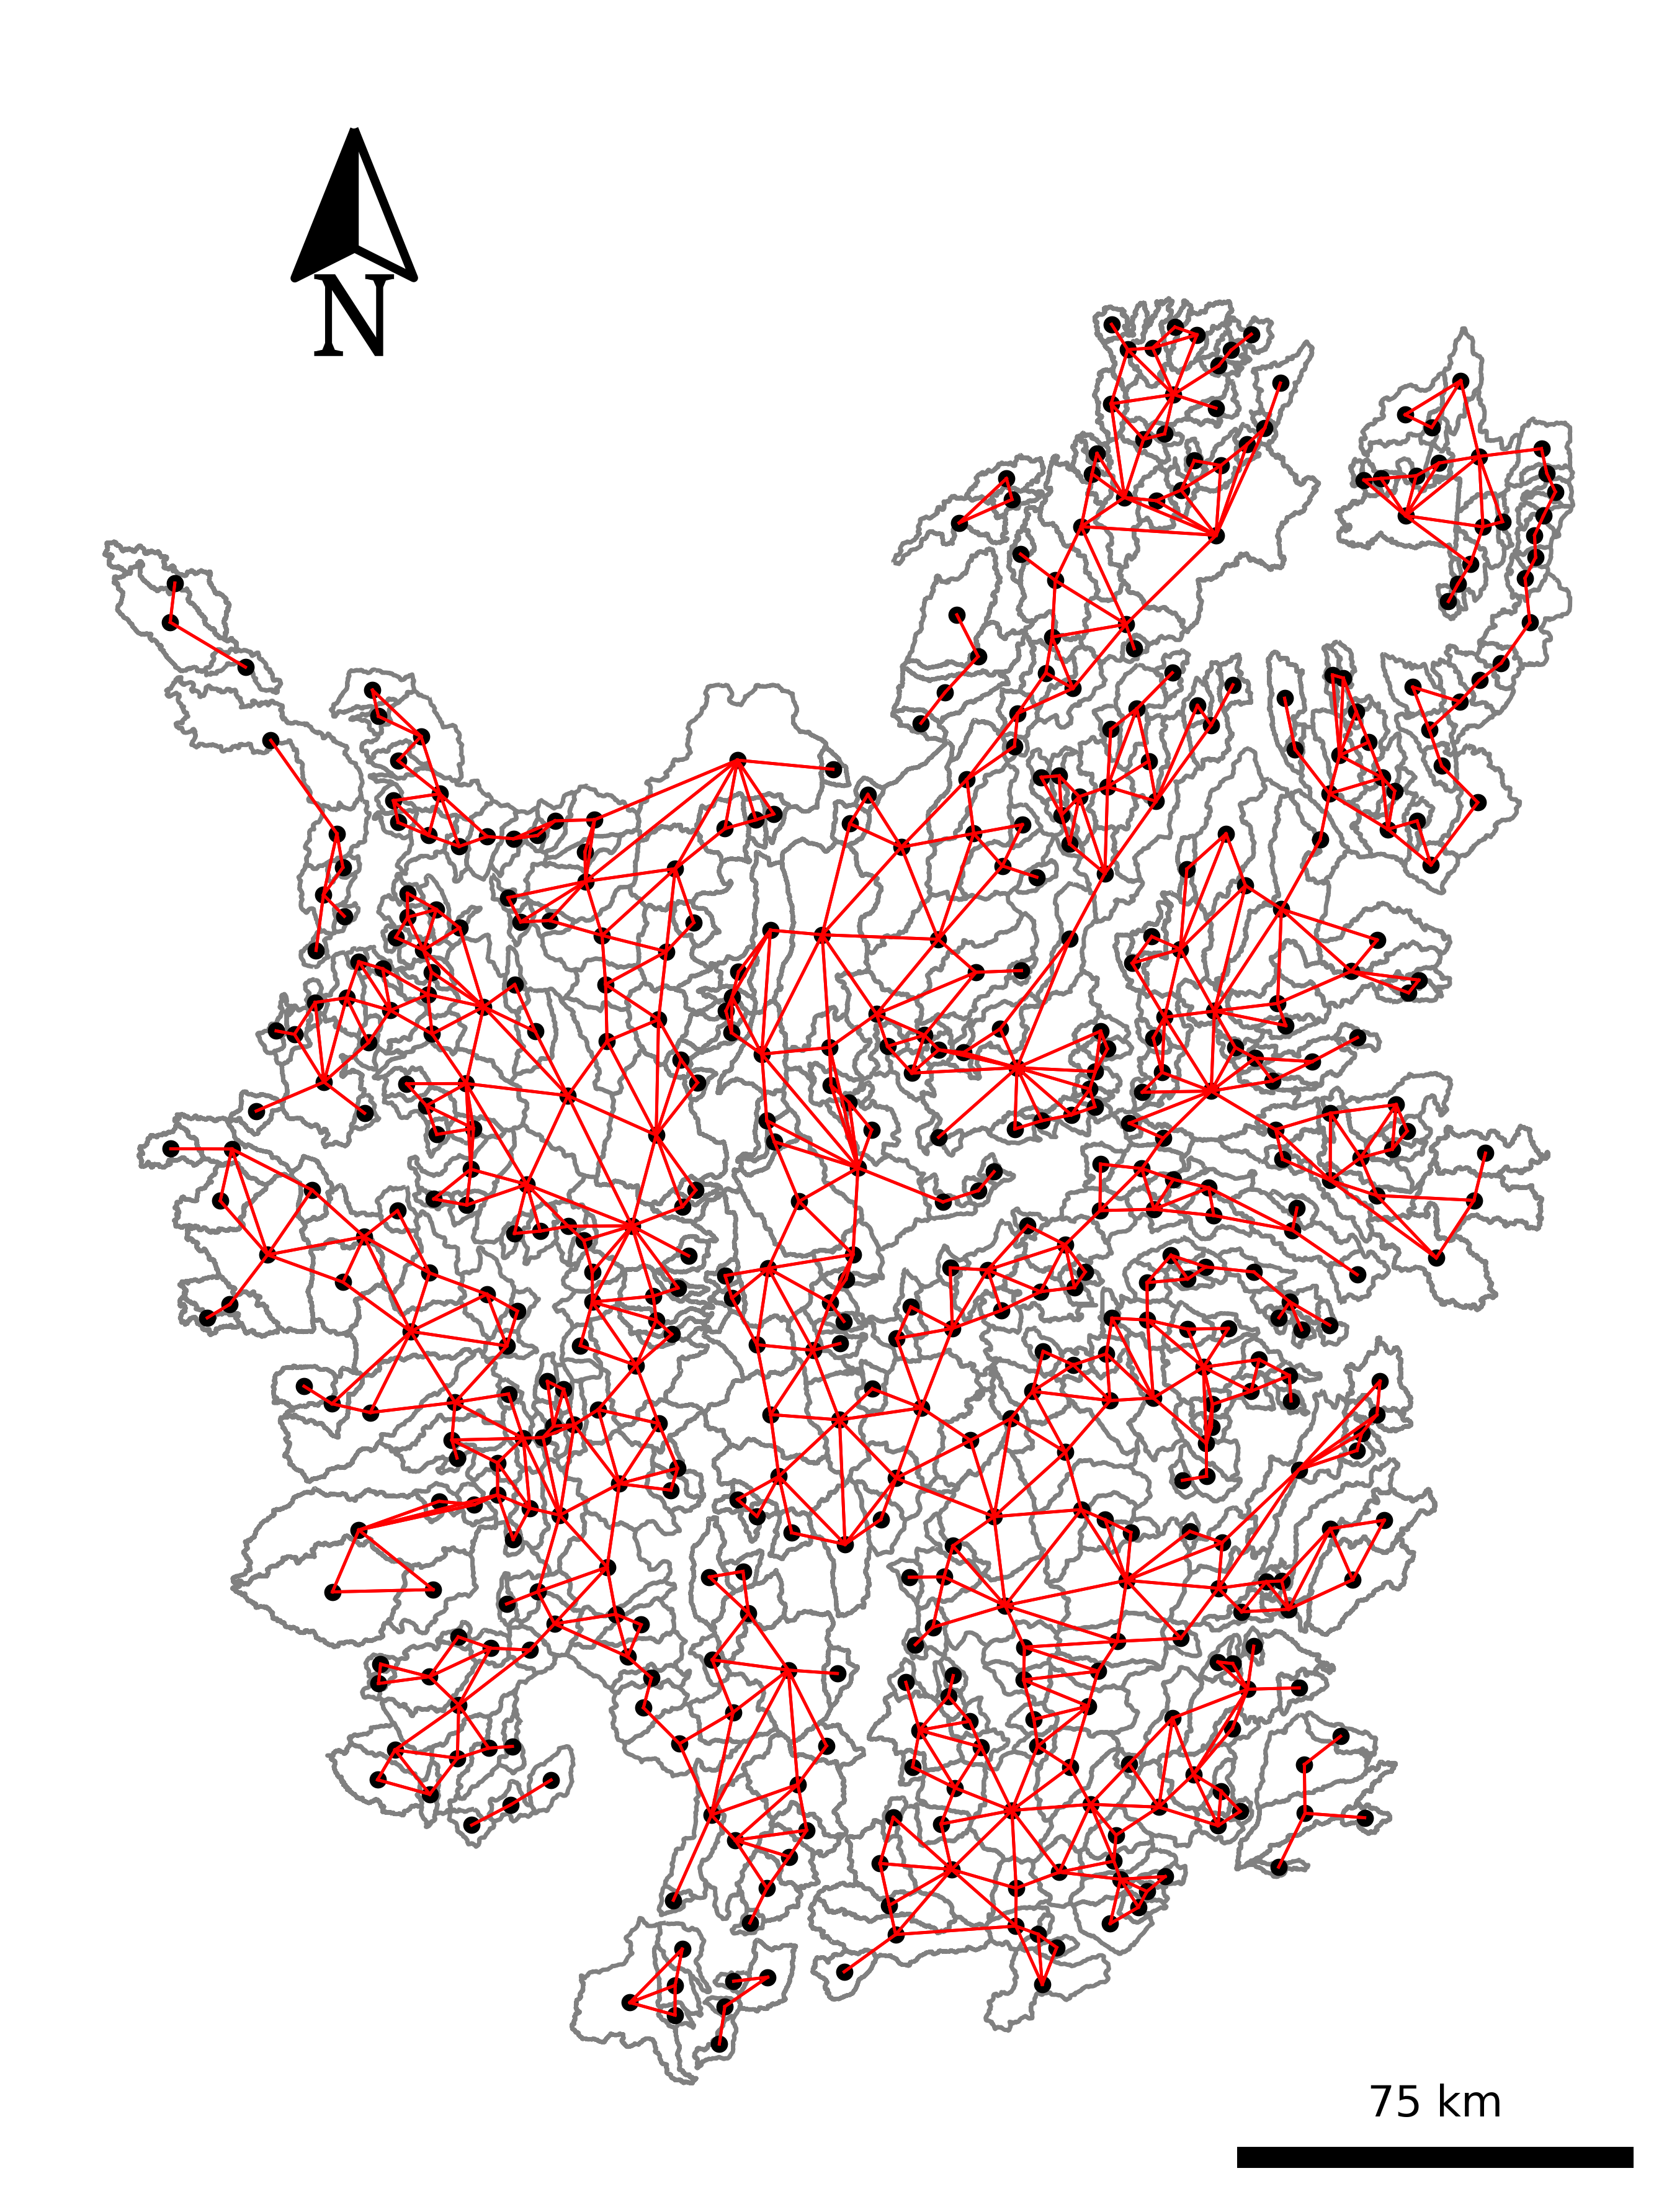
\includegraphics[width=0.45\textwidth]{Fig2A.png}
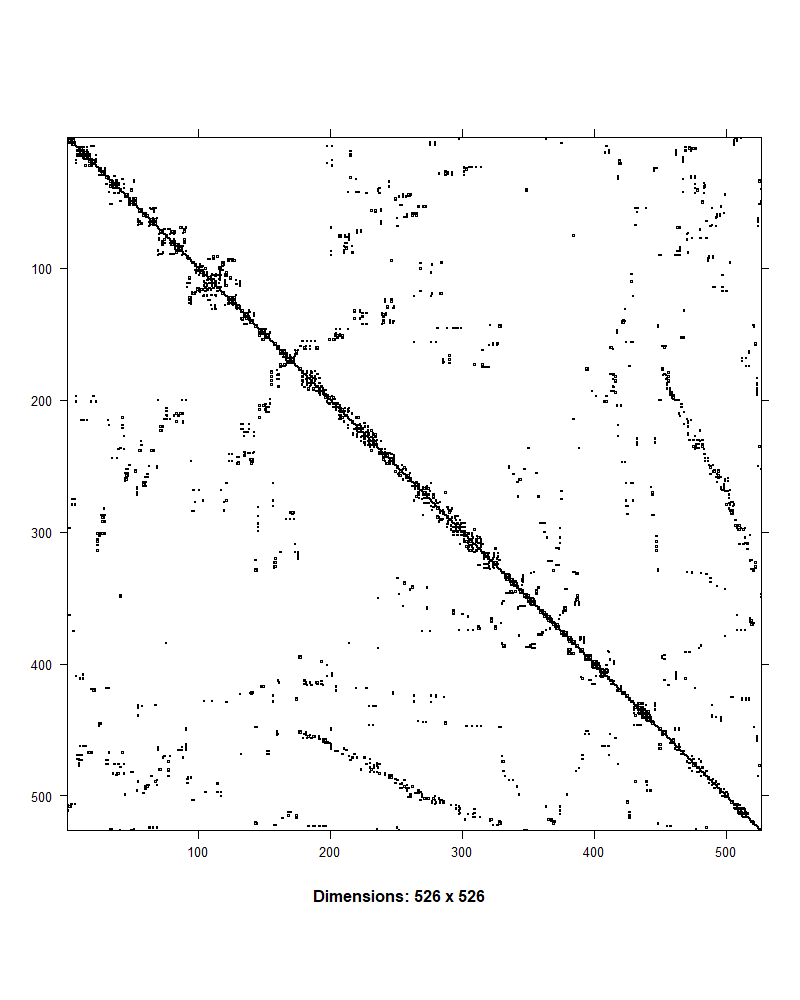
\includegraphics[width=0.45\textwidth]{Fig2B.png}
\caption{Spatial contiguity weight matrix (queen). (A) Adjacency matrix representation. (B) Covariance matrix visualization.}
\label{Fig2}
\end{figure}


\section{Results}\label{sec4}

We present the results from a series of five hierarchical models designed to assess landslide susceptibility in the northern Colombian Andes. This series follows a progression of increasing complexity to systematically evaluate the impact of spatial effects. We begin with a simple Poisson model (M1) to estimate the predictor effects on landslide counts, assuming spatial independence. We then introduce a multilevel model (M2) that incorporates random intercepts at the upper level (basins). We further extend this structure by modeling spatial dependence at the lower level (catchments) with Conditional Autoregressive (CAR) structures in the random effects. We explore three increasingly flexible spatial models: the Intrinsic Conditional Autoregressive (ICAR) model (M3), the Besag--York--Molli\'{e} (BYM) model (M4), and the Leroux model (M5). This progression of models, from a simple non-spatial baseline to different spatial formulations, enhances the capacity to represent both large-scale spatial heterogeneity and local spatial dependency, providing a more comprehensive framework for capturing the spatial complexity of landslide processes.

\subsection{Model 1: Simple Poisson model}\label{subsec41}

Our simplest model (M1) is a standard Poisson GLM where the expected landslide count, $\lambda_i$, is modeled as a function of our three predictors, including an offset term to account for the area of each catchment ($A_i$). The linear predictor is defined as:

\begin{equation}
\eta_i = \beta_0 + \beta_1 Rd_i + \beta_2 S_i + \beta_3 H_i + \log(A_i)
\end{equation}

where $Y_i$ is the number of landslides in catchment $i$. This count is modeled as a function of days with rainfall exceeding 20 mm ($Rd$), mean catchment slope ($S$), and mean catchment elevation ($H$), and includes an offset term, $\log(A_i)$, to normalize for the area ($A_i$) of each catchment.

This simple Poisson model reveals significant positive relationships between landslide occurrence and all predictors. After exponentiating the model coefficients to obtain Rate Ratios (RR), we found that for each additional day with rainfall exceeding 20 mm, the expected landslide count increases by a factor of 1.16 (RR = 1.16, $p < 0.05$). For each one-degree increase in mean catchment slope, the expected count multiplies by 1.85 (RR = 1.85, $p < 0.01$). For each one-meter increase in mean catchment elevation, the expected count increases by a factor of 1.51 (RR = 1.51, $p < 0.01$). These results highlight mean slope as the predictor with the strongest effect on landslide rates.

The Moran’s statistic indicates residual spatial autocorrelation, which may reduce the reliability of the model estimates, and suggests the need for additional spatial effects or a more sophisticated spatial structure. This strong spatial clustering in the residuals (Fig. 3) is a clear statistical signal of unmodeled physical processes. It indicates that our predictors (slope, rain, elevation) are insufficient on their own to explain where landslides are concentrated, strongly suggesting the presence of an underlying, spatially-organized geological or soil factor.

\begin{figure}[h]
\centering
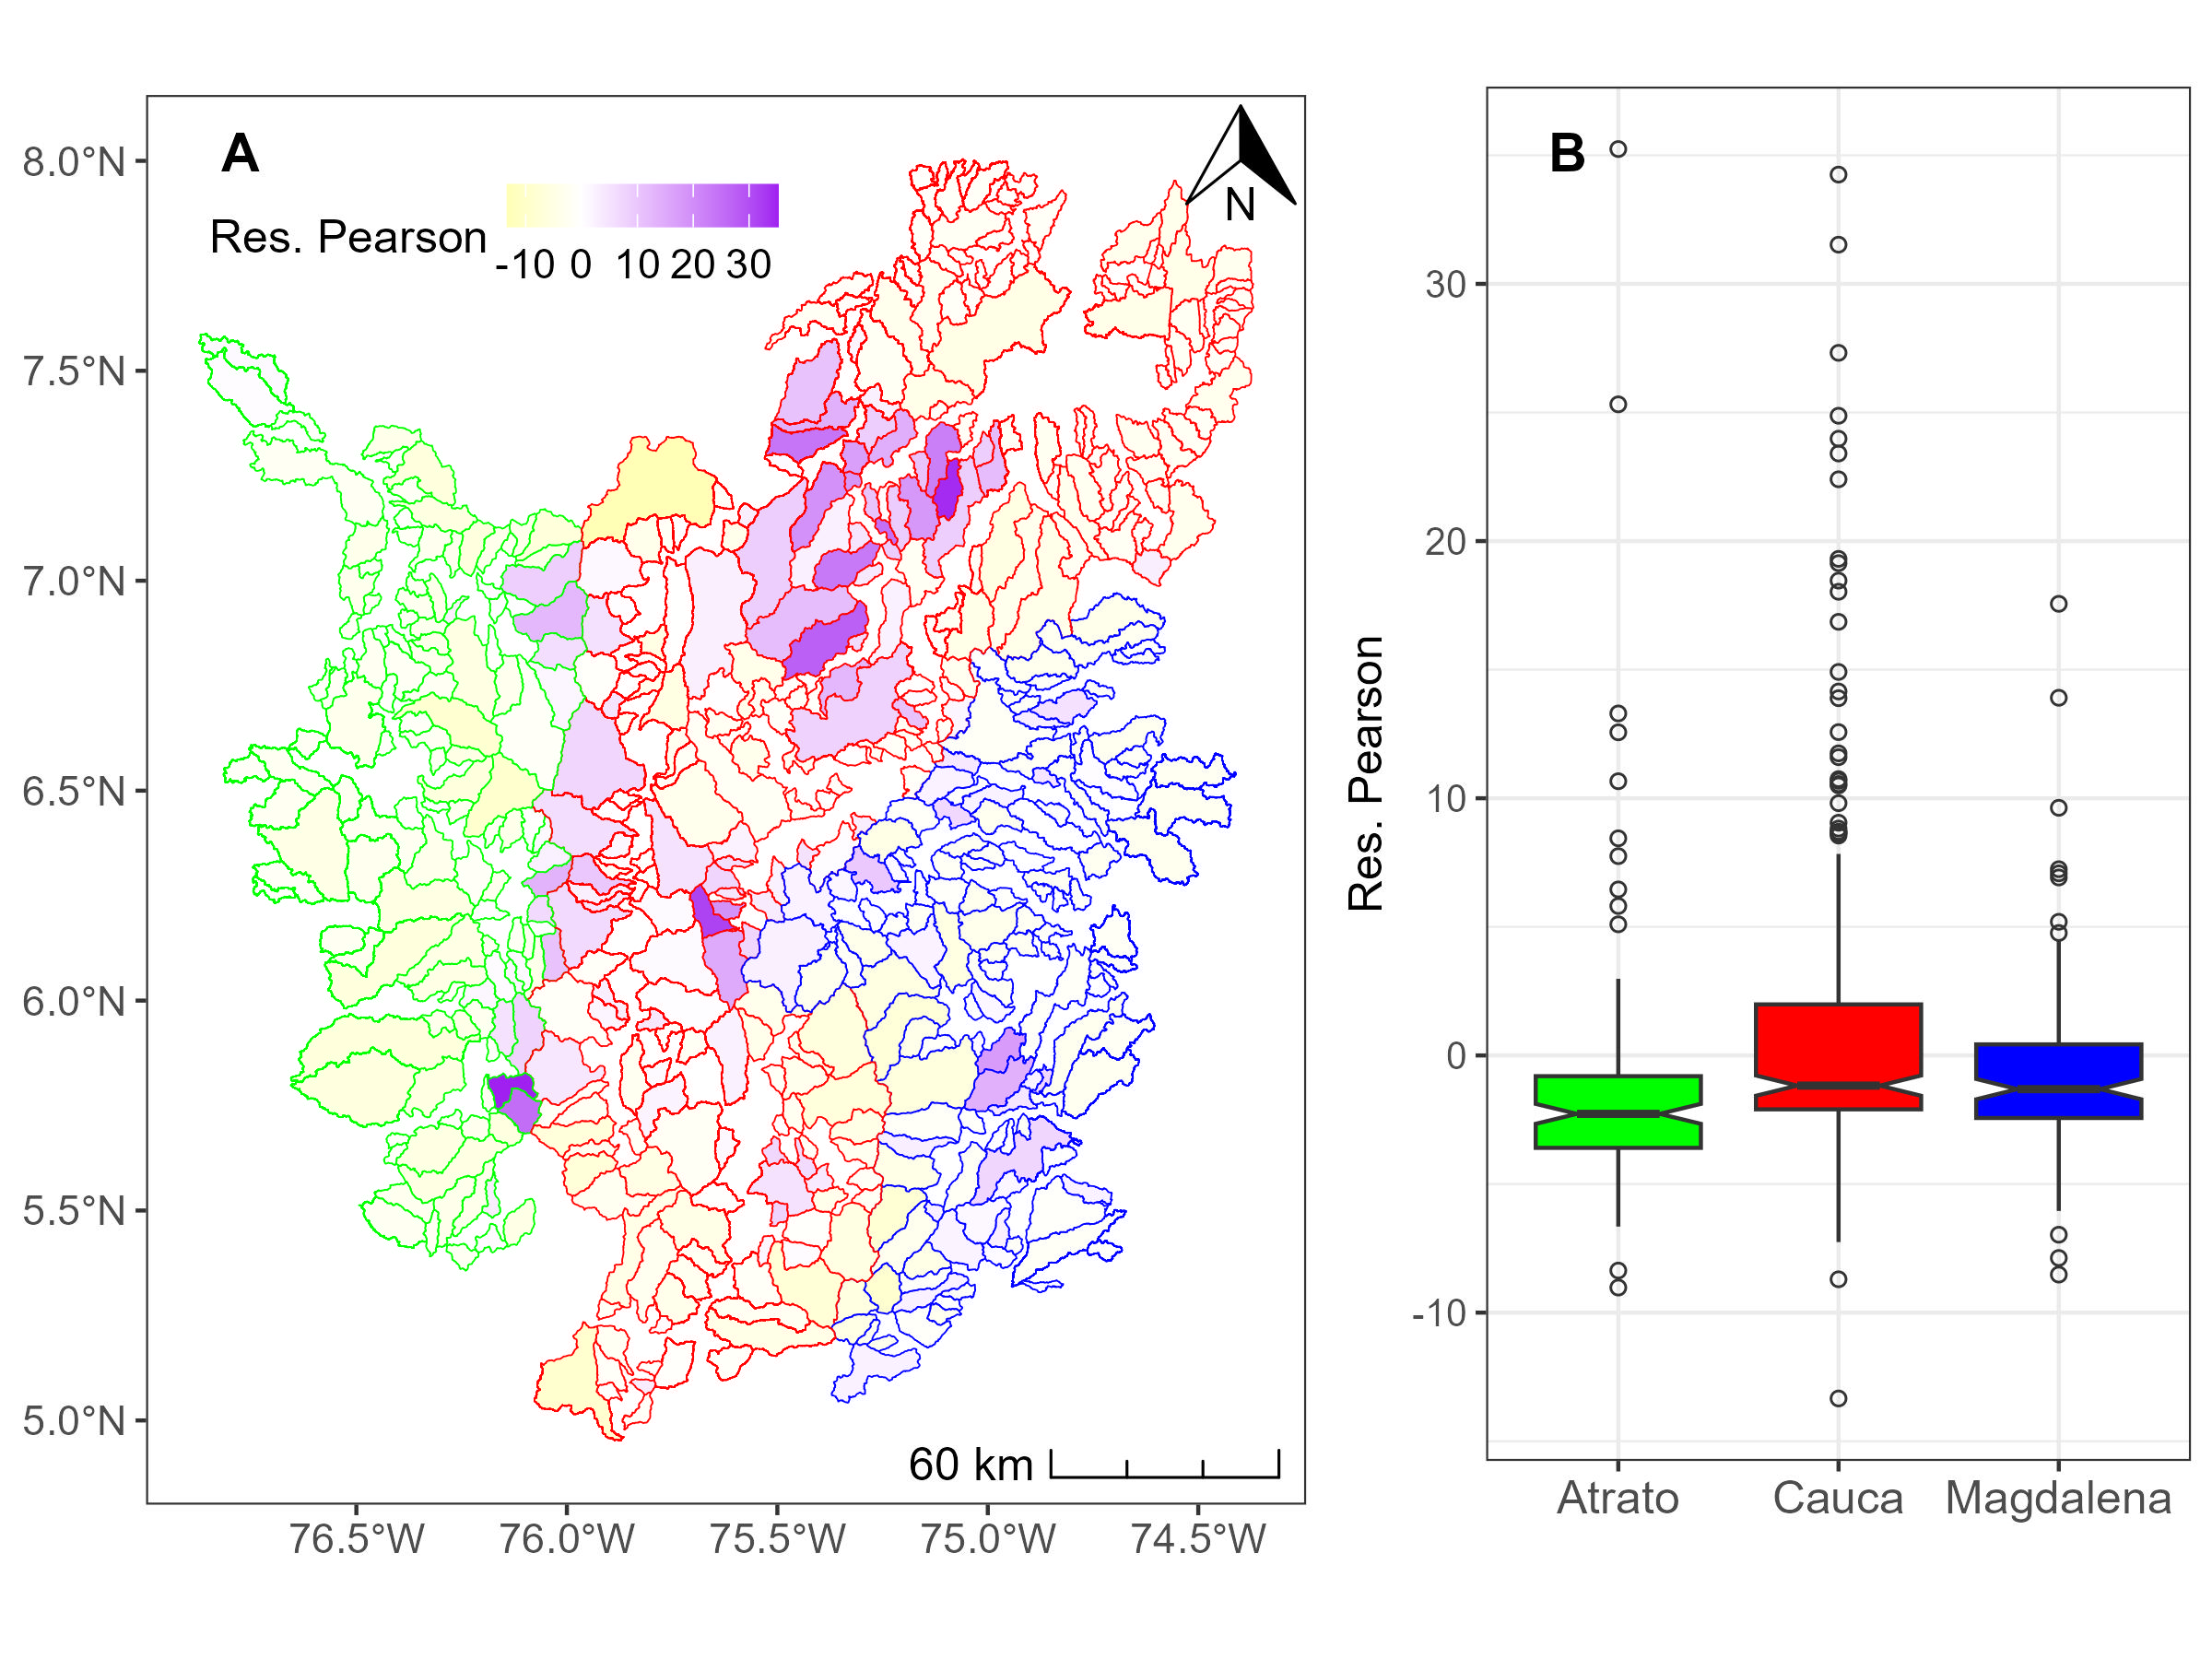
\includegraphics[width=0.8\textwidth]{Fig3.jpg}
\caption{Model M1 – Standard Poisson. (A) Observed landslide counts per catchment in the northern Colombian Andes. (B) Standardized Pearson residuals from the baseline Poisson model without spatial effects (M1). The residuals show pronounced spatial clustering, indicating strong residual spatial autocorrelation. The high Moran’s Index (MI = 0.513) supports the presence of unaccounted spatial structure in the model.}
\label{Fig3}
\end{figure}


\subsection{Model 2: Random intercept model at basin level}\label{subsec42}

The random intercept model at basin level includes an unstructured latent random effect at the basin level (Cauca, Magdalena, and Atrato):

\begin{equation}
Y_{ij} \sim Poisson(\lambda_{ij}), \lambda_{ij} = \exp(\beta_0 + \beta_1 Rd_{i} + \beta_2 S_i + \beta_3 H_i + u_j + \log(A_i))
\end{equation}

where $u_j$ is the random intercept for basin $j$, capturing unobserved heterogeneity (i.e., systematic baseline differences) among the known basins.

Prior to modeling, all predictors were standardized (e.g., scaled to a mean of 0 and a standard deviation of 1). After fitting the model, all three predictors showed credible positive effects. In particular, slope and elevation show relatively high posterior means (0.661 and 0.485, respectively), suggesting strong contributions to landslide susceptibility. While the effect of rainfall days is small (0.299), it remains positive.

The global intercept of the model represents the average baseline landslide susceptibility for the entire study area (i.e., the mean across all 526 catchments). The basin-specific random effects are then interpreted as deviations from this overall average. Among these effects, only the Cauca basin has a positive posterior mean (0.311), indicating a higher baseline susceptibility relative to this global intercept. Conversely, the Atrato and Magdalena basins show negative or near-zero values, suggesting either inherently lower landslide activity or that their local variability is better captured by other, likely catchment-level predictors.

This M2 formulation (DIC = 13,228; WAIC = 10,296) shows a notable improvement in model fit over the non-spatial M1 benchmark (DIC = 13,649; WAIC = 10,295). Furthermore, the residual Moran’s Index (MI) decreases substantially from 0.513 (M1) to 0.447 (M2), indicating that incorporating basin-level heterogeneity successfully reduced some of the residual spatial autocorrelation. This reduction shows that some of the spatial clustering is due to large-scale regional differences between basins (e.g., the Cauca basin being inherently more susceptible). However, the still-high Moran’s I confirms that most of the spatial structure exists at a local, catchment-to-catchment scale.

\begin{figure}[h]
\centering
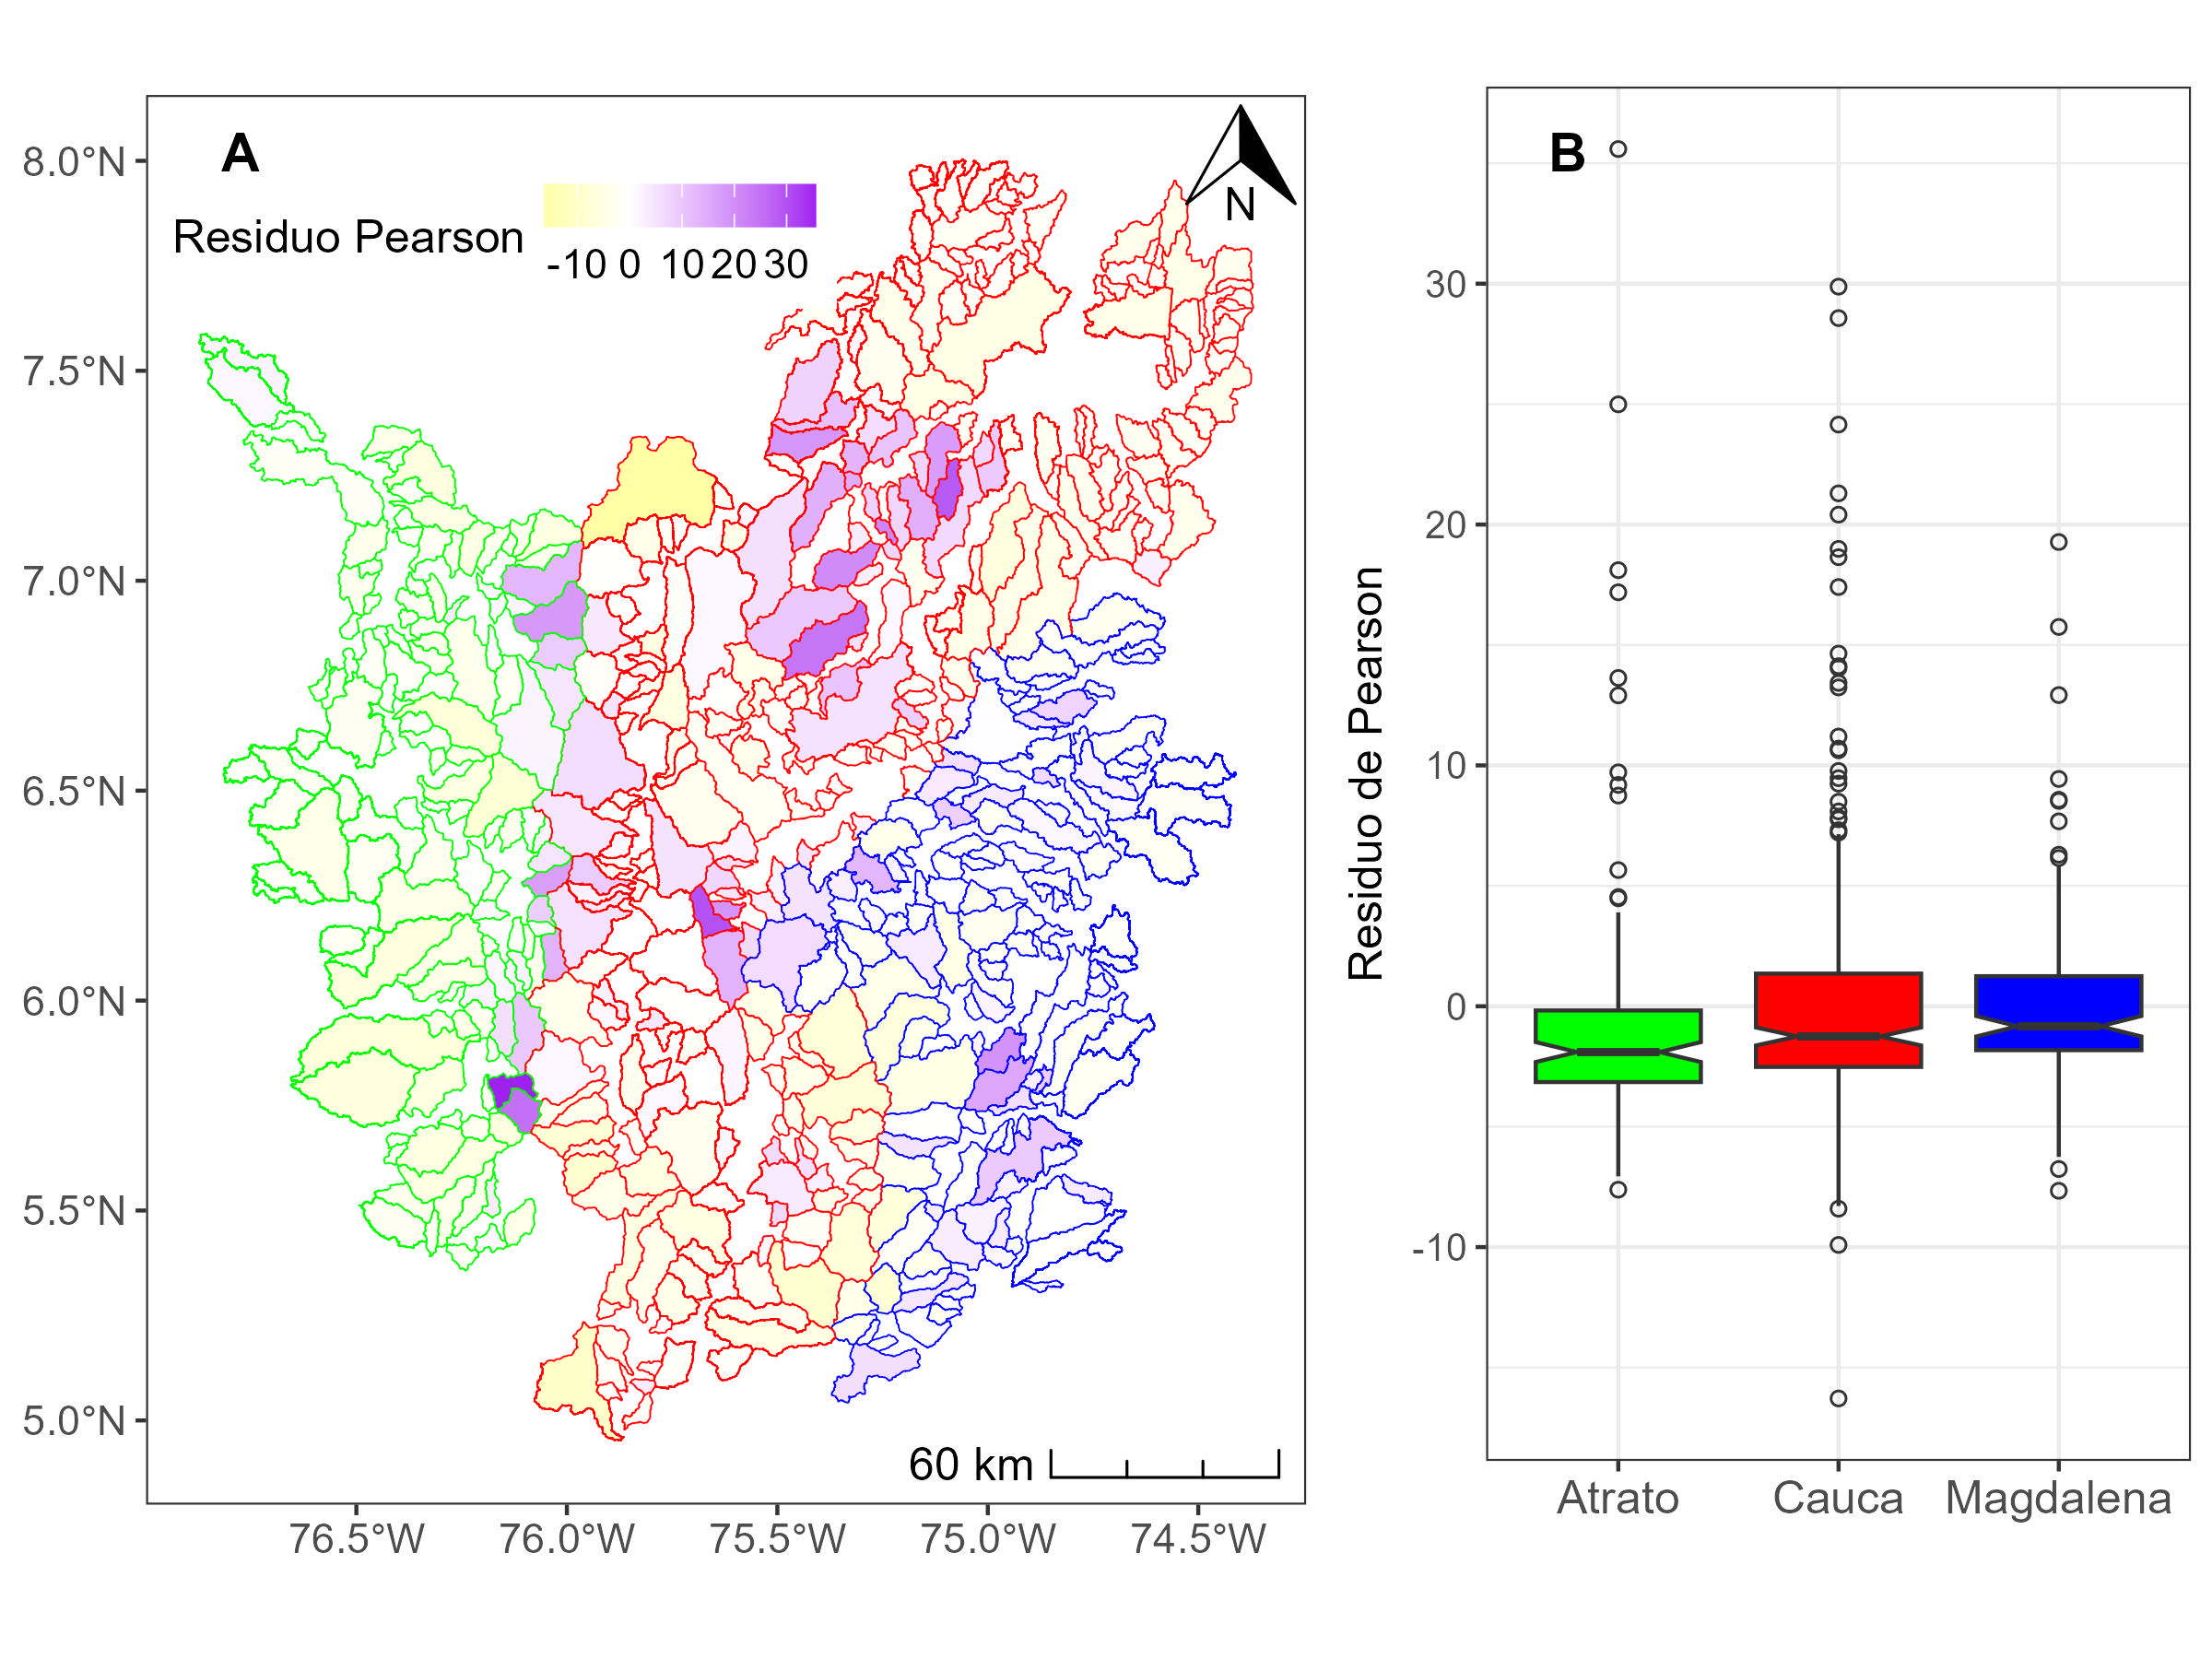
\includegraphics[width=0.8\textwidth]{Fig4.jpg}
\caption{Model M2 – Multilevel Poisson with Random Effects at Basin Level. (A) Pearson residuals from the multilevel Poisson model including an unstructured random intercept at the basin level (Atrato, Cauca, Magdalena). (B) Distribution of residuals by basin. While the inclusion of upper-level heterogeneity reduces some regional variability, spatial clustering of residuals remains apparent—especially in the Cauca basin—suggesting unaccounted local spatial dependence. The residual Moran’s Index (MI = 0.447) confirms the persistence of moderate spatial autocorrelation, thus justifying the need for models incorporating spatial dependency at the catchment level.}
\label{Fig4}
\end{figure}


\subsection{Model 3: ICAR model}\label{subsec43}

To account for local spatial dependency at the TMU level, we test the Intrinsic Conditional Autoregressive (ICAR) model:

\begin{equation}
Y_i \sim Poisson(\lambda_i), \lambda_i = \exp(\beta_0 + \beta_1 Rd_i + \beta_2 S_i + \beta_3 H_i + u_i)
\end{equation}

where $u_i$ is a spatial random effect that follows an ICAR structure. The ICAR prior for $u_i$ is defined as:

\begin{equation}
u_i | \{u_j : j \neq i\} \sim N \left( \frac{1}{n_i} \sum_{j \in N(i)} u_j, \frac{\sigma^2}{n_i} \right)
\end{equation}

which ensures that spatially neighboring units have similar random effects, imposing smoothness on the spatial structure.

In terms of fixed effects, the posterior means for slope (0.727) and elevation (0.832) remain credibly positive, confirming their effect on landslide susceptibility. The estimate for rainfall days (1.355) is substantially higher than in previous models.

The random intercepts at the basin level are more spread out in this model: Cauca continues to exhibit a strong positive effect (0.757), whereas Atrato (-0.521) and Magdalena (-0.235) are negative, indicating that basin-level heterogeneity is not fully explained.

Although the DIC (2626) and WAIC (2657) are slightly higher than in the BYM and Leroux models, the residual Moran’s Index (MI) drops to -0.254, the lowest across all models tested. This behaviour of the spatial model is controlled by the precision of the TMU-level effect, a hyperparameter that dictates how much the spatial random effect is allowed to vary between adjacent catchments. A high precision forces neighbors to be very similar (i.e., high smoothing), while a low precision allows for more local variability. We estimated a precision of 5.253. As precision is the inverse of variance (1/5.253 $\approx$ 0.19), this value indicates a relatively low variance, reflecting that the model is applying a moderate level of spatial smoothing across neighboring units.

\begin{figure}[h]
\centering
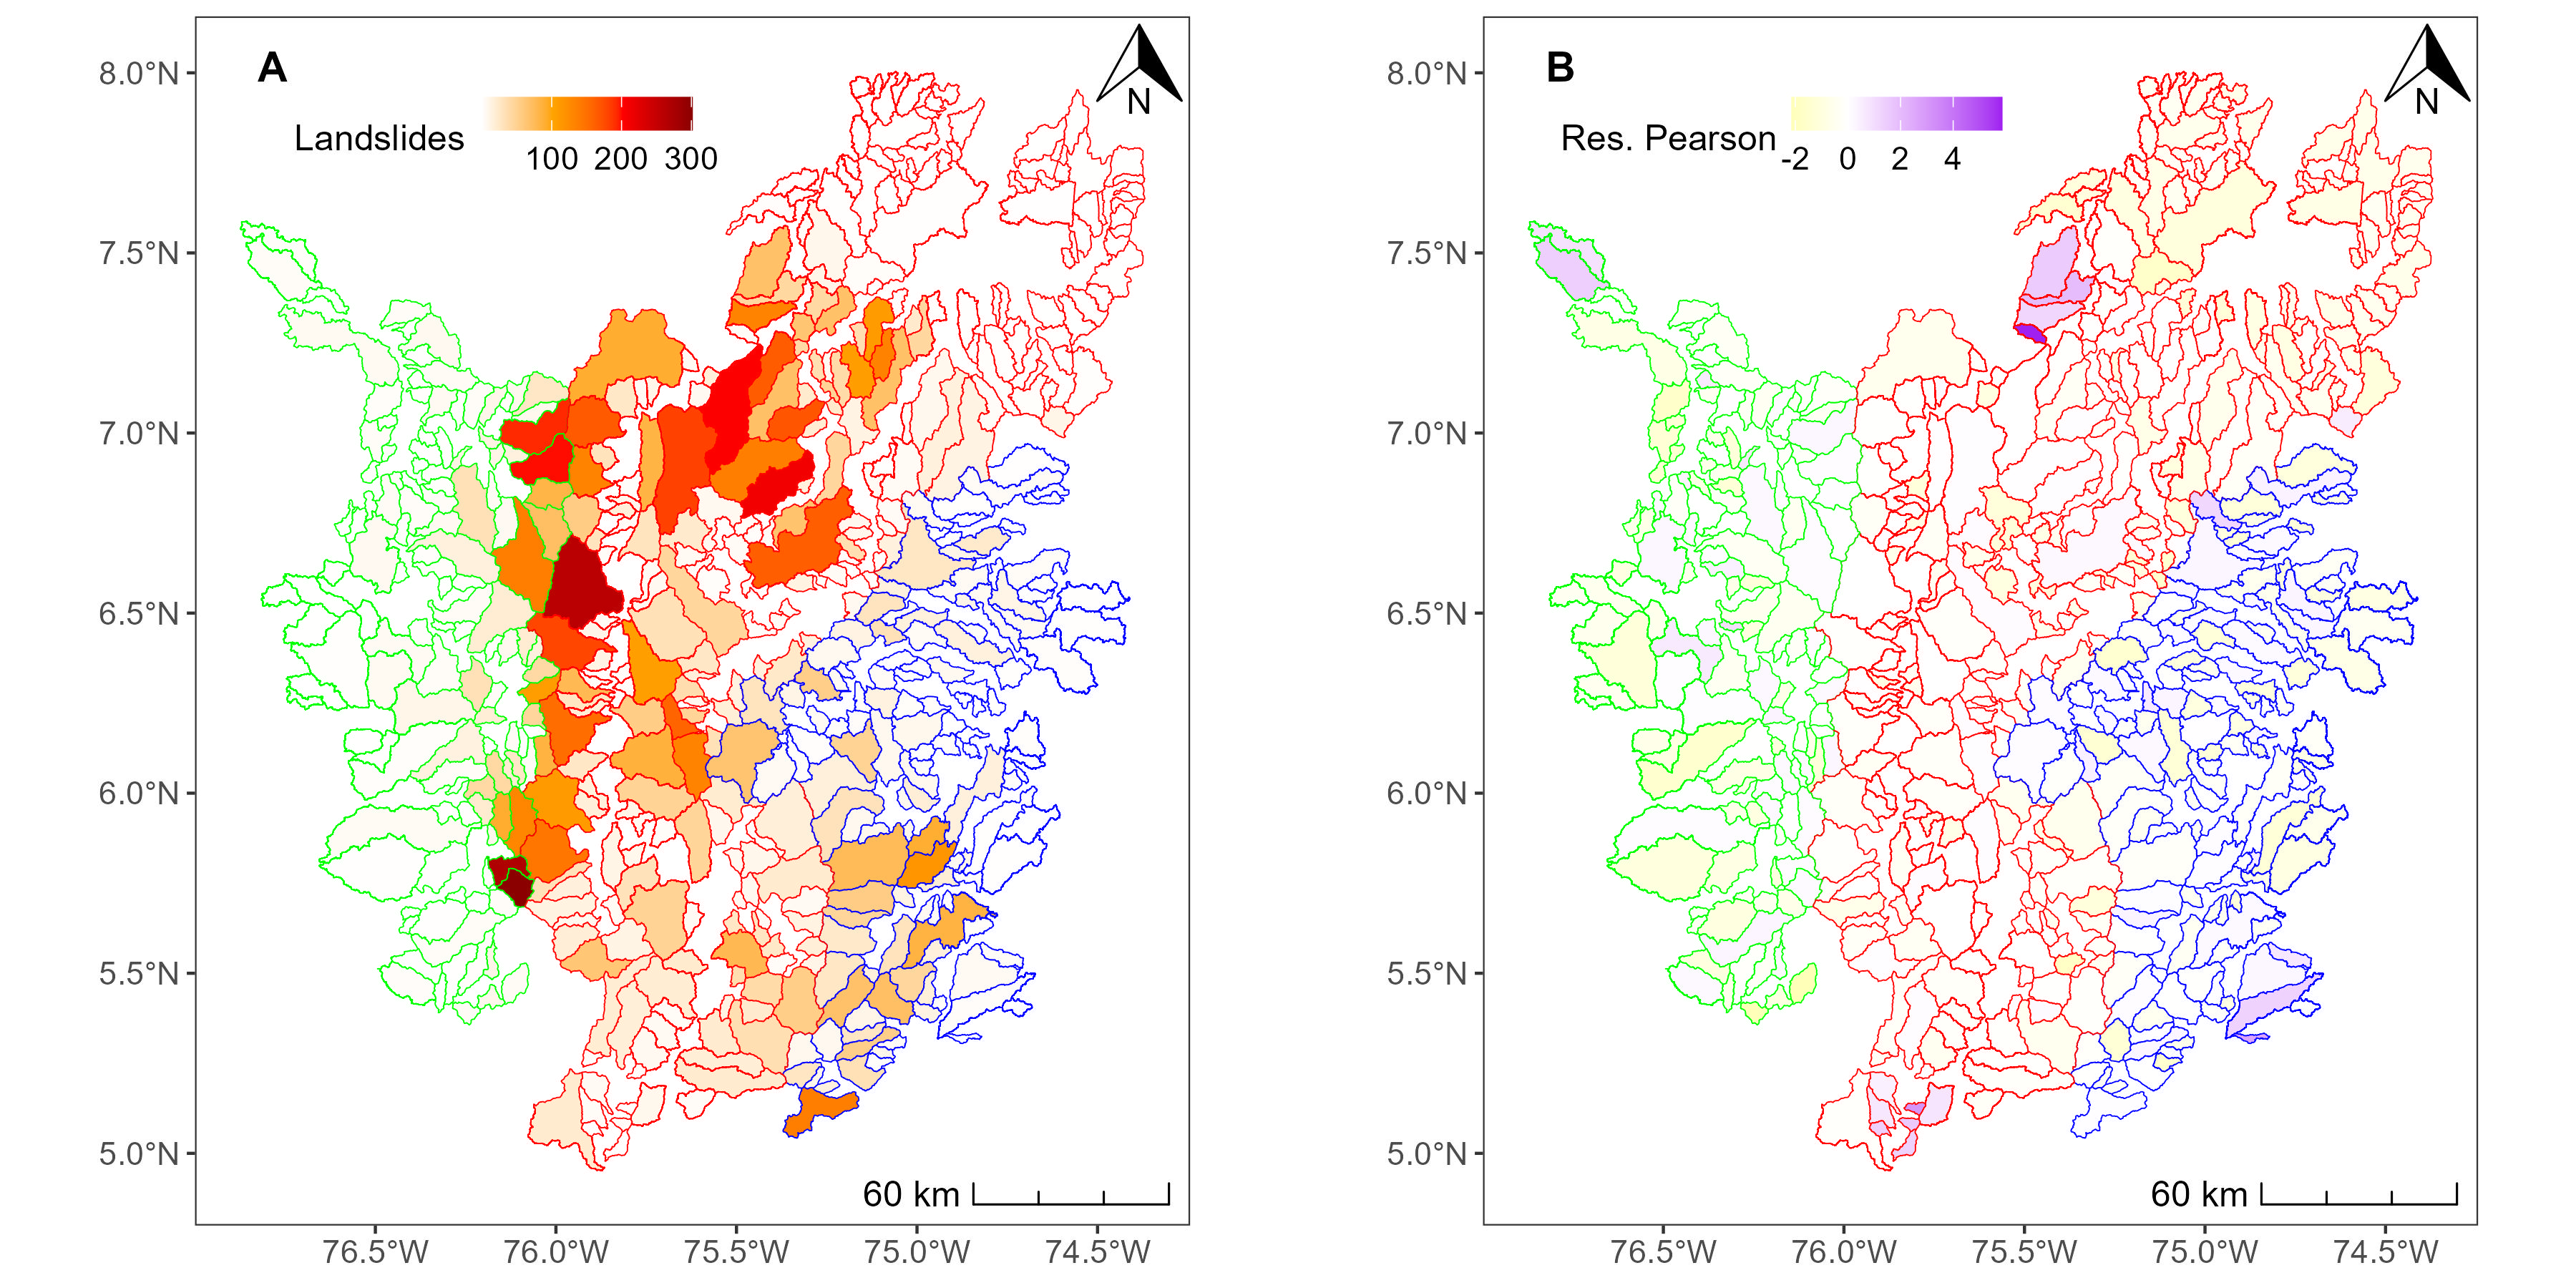
\includegraphics[width=0.8\textwidth]{Fig5.jpg}
\caption{Model M3 – Intrinsic Conditional Autoregressive (ICAR). (A) Predicted landslide counts using the ICAR model at the catchment level. (B) Pearson residuals after including a spatially structured random effect via an ICAR prior. The spatial pattern of residuals is substantially reduced (MI = –0.254), indicating that the model effectively captures local spatial dependence in landslide occurrences.}
\label{Fig5}
\end{figure}


\subsection{Model 4: Besag--York--Molli\'{e} (BYM) model}\label{subsec44}

The BYM model combines spatially structured and unstructured random effects:

\begin{equation}
Y_i \sim Poisson(\lambda_i), \lambda_i = \exp(\beta_0 + \beta_1 Rd_i + \beta_2 S_i + \beta_3 H_i + u_i)
\end{equation}

where $u_i$ includes both structured and unstructured components, accounting for overdispersion and unobserved heterogeneity.

Regarding fixed effects, all predictors have positive coefficients. Slope and elevation remain credibly non-zero, with posterior means of 0.745 and 0.408, respectively, in the R-INLA implementation. The effect of rainfall days is reduced compared to the ICAR model (now 0.121).

The estimated precision for the TMU-level effects is 1.42, corresponding to a posterior variance of approximately 0.704, which confirms residual overdispersion, but lower than in the ICAR-only model (variance = 0.19). The upper-level (basin) random effects are largely attenuated in this specification, with near-zero posterior means for all three basins: Atrato (-0.001), Cauca (0.001), and Magdalena (0.000), indicating that most of the regional variation has been absorbed by the flexible structure at the TMU level.

Model fit remains favorable, with a DIC of 2524 and WAIC of 2453, showing only marginal increases in complexity relative to the ICAR model. The residual Moran’s Index (MI) is -0.111, suggesting that the model effectively mitigates residual spatial autocorrelation.

\begin{figure}[h]
\centering
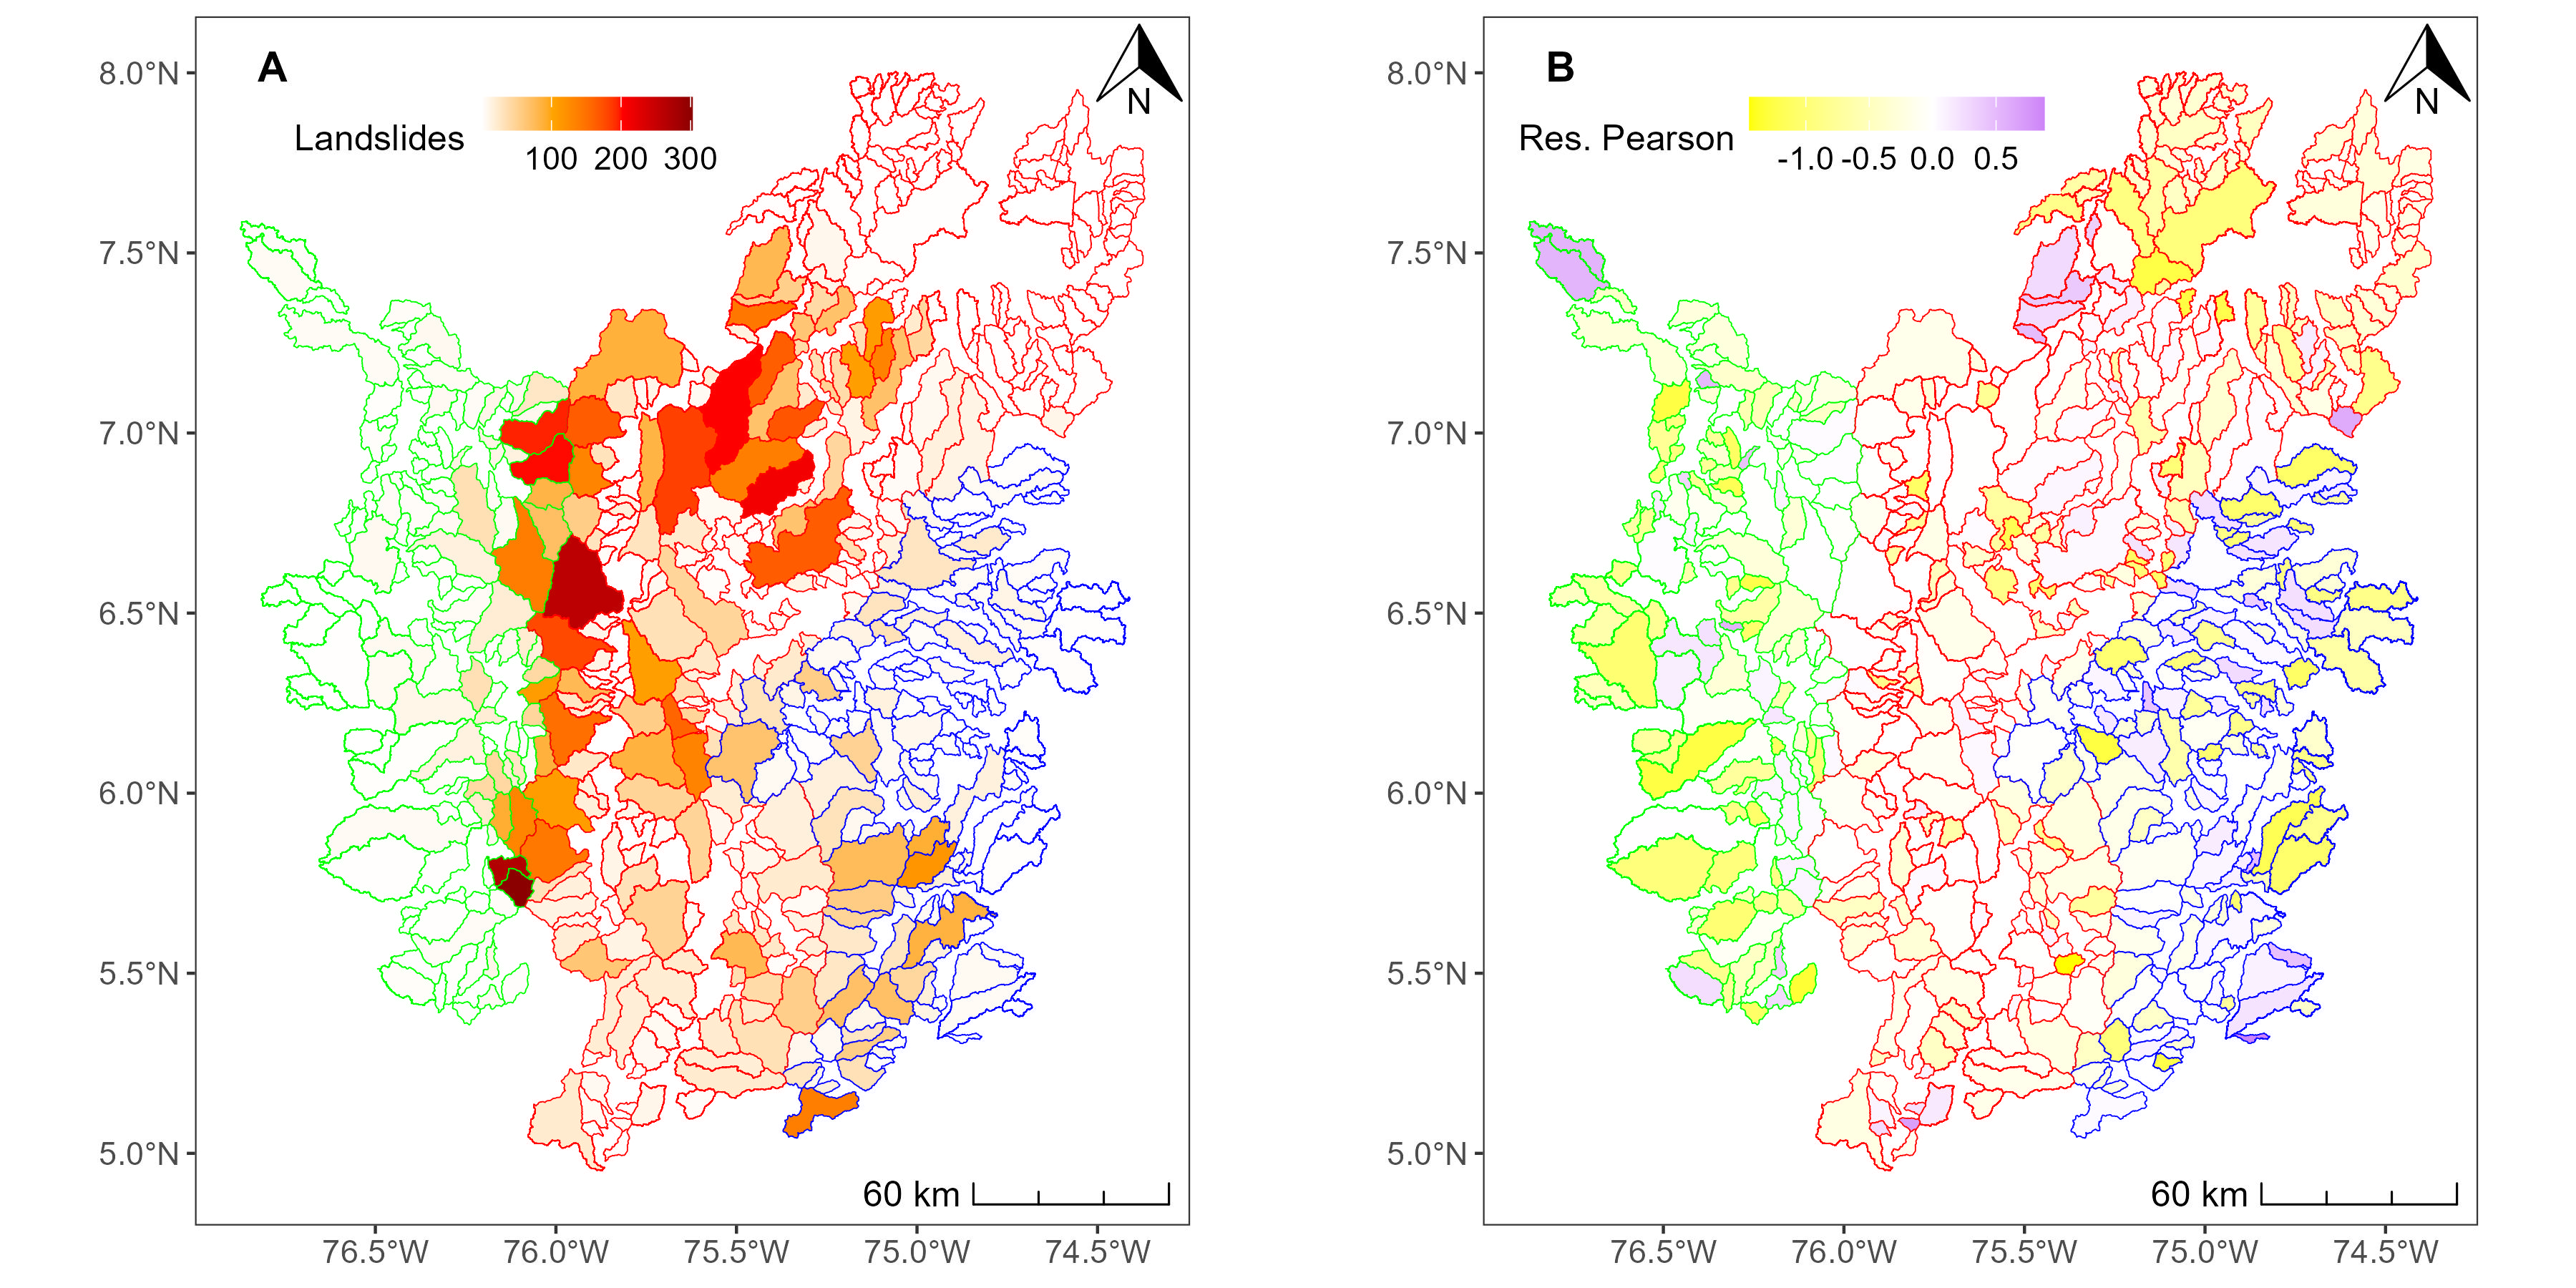
\includegraphics[width=0.8\textwidth]{Fig6.jpg}
\caption{Model M4 – Besag–York–Mollié (BYM). (A) Predicted landslide counts under the BYM model, which includes both structured and unstructured random effects at the TMU level. (B) Residuals show moderate spatial randomness, with most high values removed and MI reduced to 0.073. The BYM model balances spatial smoothing and overdispersion control, improving model fit relative to ICAR.}
\label{Fig6}
\end{figure}


\subsection{Model 5: Leroux model}\label{subsec45}

Lastly, we evaluate the Leroux model, incorporating spatial independence at the upper level, and a parameter to control the degree of spatial smoothing:

\begin{equation}
Y_i \sim Poisson(\lambda_i), \lambda_i = \exp(\beta_0 + \beta_1 Rd_i + \beta_2 S_i + \beta_3 H_i + u_i)
\end{equation}

where $u_i$ follows a Leroux prior:

\begin{equation}
u_i \sim N \left( \rho \sum_{j \in N(i)} w_{ij} u_j, (1 - \rho) \sigma^2 \right)
\end{equation}

with $\rho$ controlling the balance between spatial dependence and independence, allowing flexibility in the spatial structure.

The posterior estimates for the fixed effects remain credibly positive. Both slope and elevation retain significant contributions to landslide susceptibility, with posterior means of 0.818 and 0.628, respectively. In contrast, the effect of rainfall days remains low and statistically ambiguous (0.134), consistent with the pattern observed in the BYM model.

The posterior mean of $\rho = 0.869$ shows a strong spatial dependency, indicating that most of the variability in the latent field is explained by the spatially structured component. This is a key physical finding, indicating that the landslide process is dominated by local spatial dependence. In physical terms, this means that nearly 87\% of the unexplained variability is structured (shared with neighbors) rather than random. This provides strong quantitative evidence that unobserved factors, such as contiguous lithology, soil type, or fracture networks, are a primary control on the landslide pattern.

The precision associated with the TMU-level effect is 0.401, corresponding to a posterior variance of approximately 2.49, which highlights a relatively high degree of overdispersion at the local level. The random intercepts at the basin level again show minimal influence, with posterior means near zero: Atrato (0.025), Cauca (-0.008), and Magdalena (-0.017), suggesting that once catchment-level spatial structure is incorporated, there is little remaining variability attributable to basin-level context.

Model performance is comparable to the BYM model, with DIC and WAIC values of 2522 and 2471, respectively. These scores confirm that the Leroux model fits the data well while maintaining interpretability and computational efficiency. Importantly, the residual Moran’s Index (MI) is -0.159, indicating that residual spatial autocorrelation has been effectively mitigated.

\begin{figure}[h]
\centering
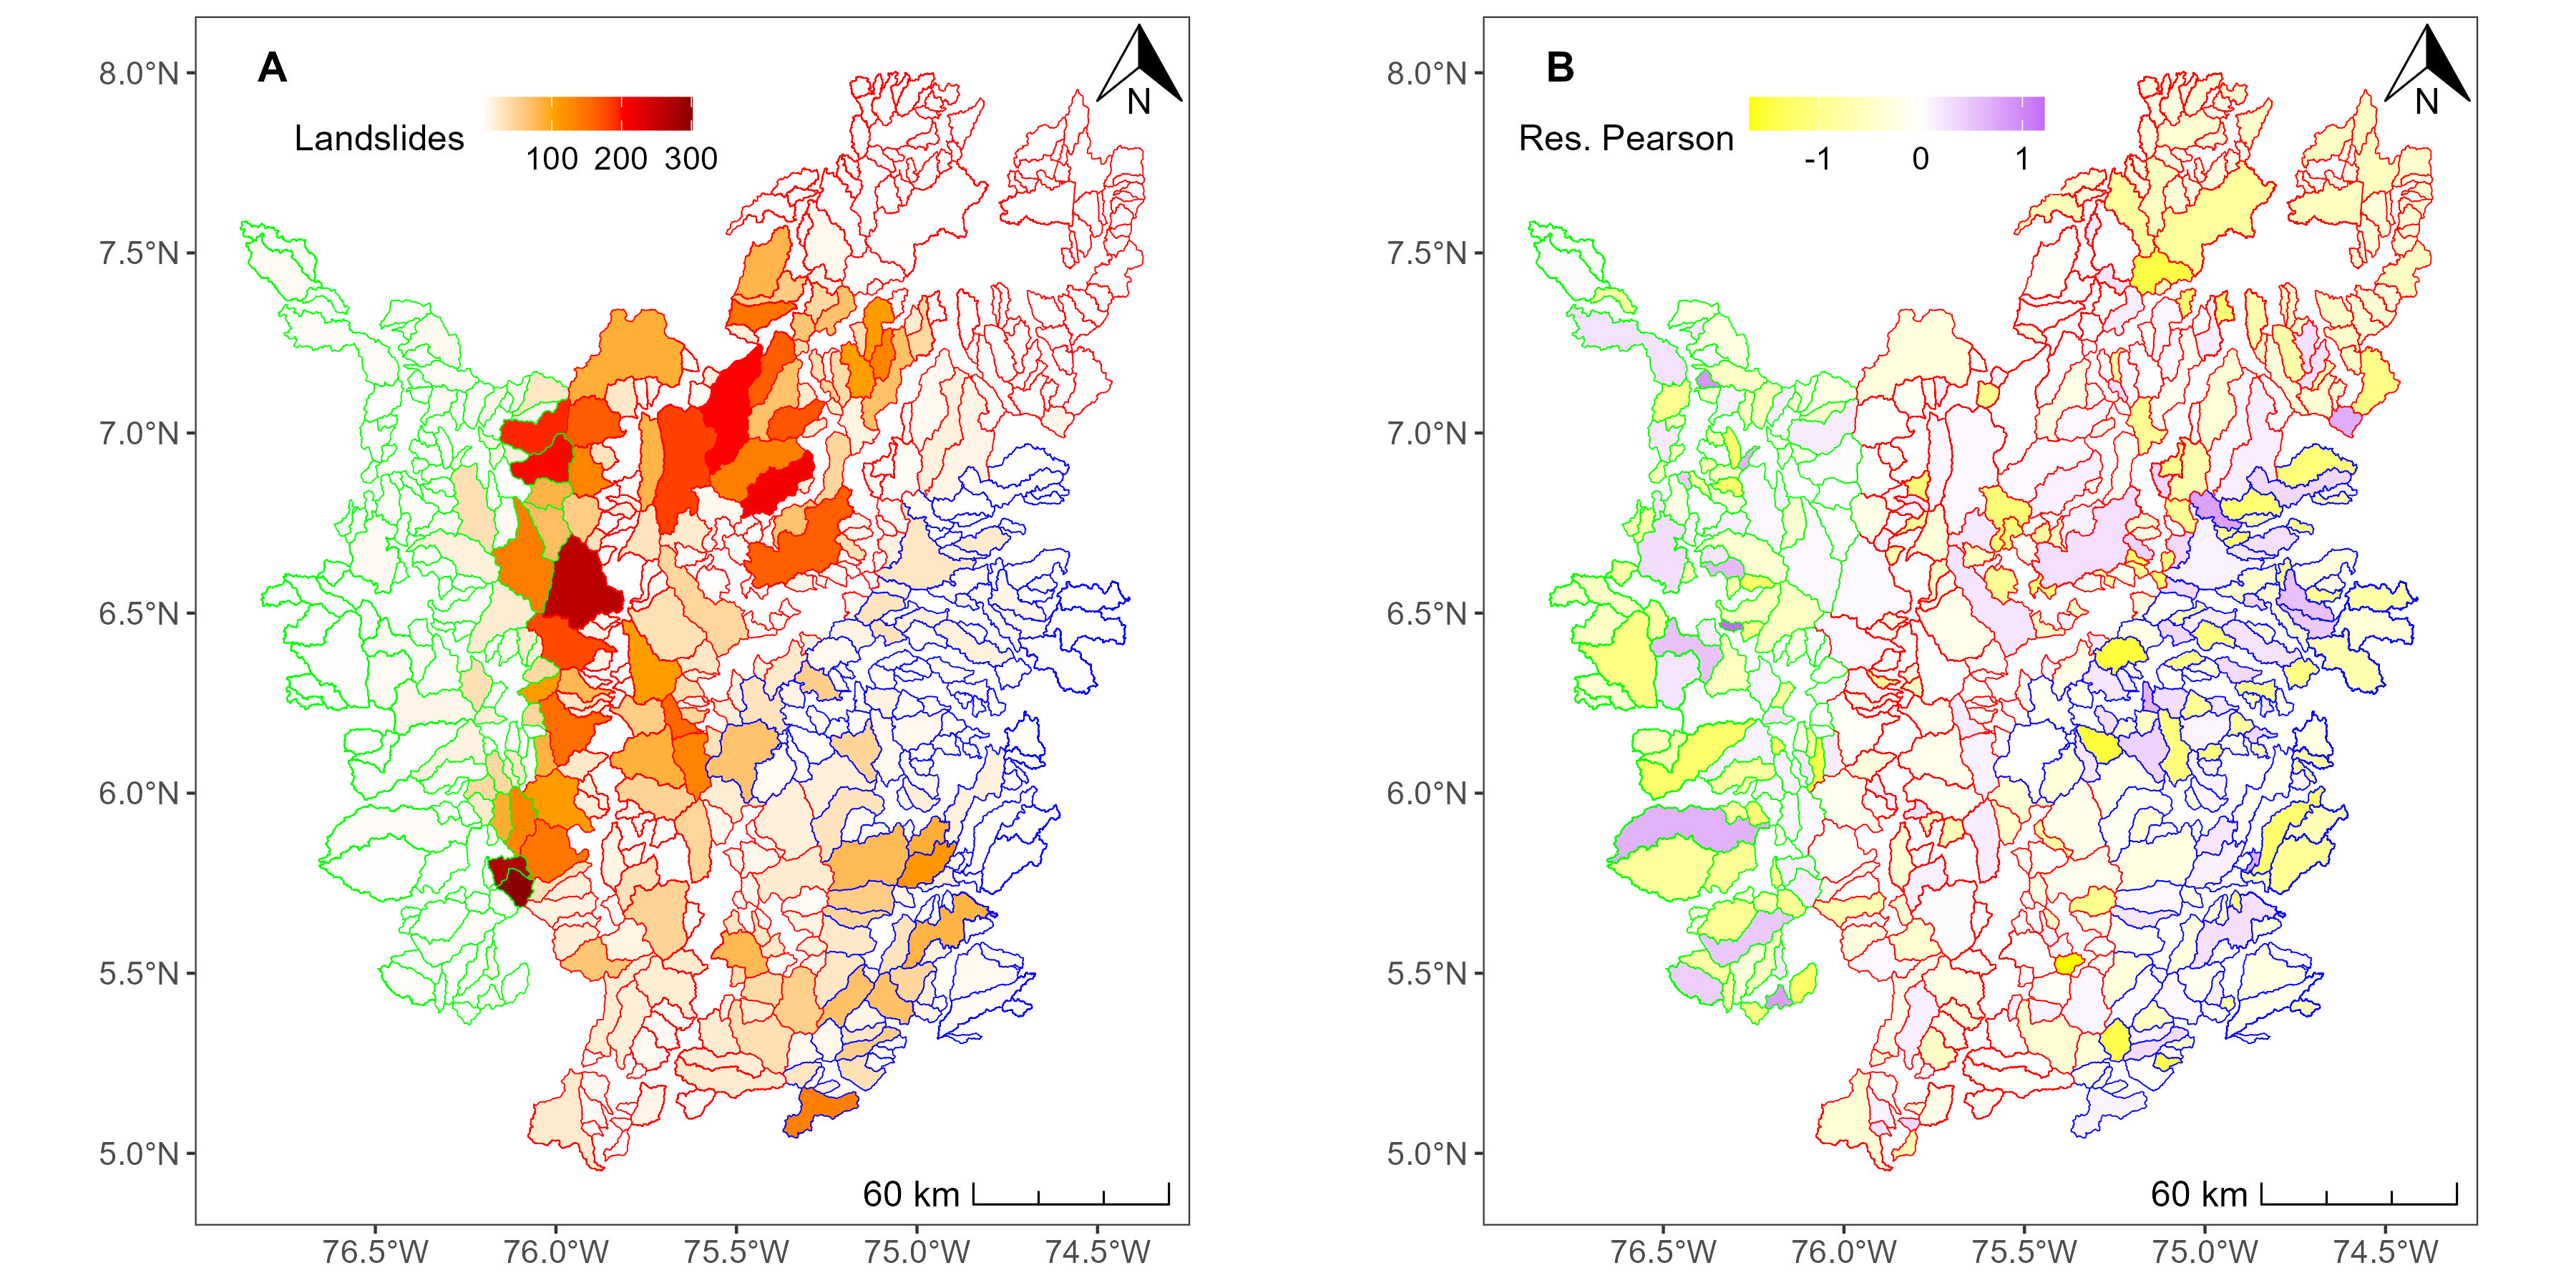
\includegraphics[width=0.8\textwidth]{Fig7.jpg}
\caption{Model M5 – Leroux.(A) Predicted landslide counts from the Leroux model, which flexibly combines spatial and unstructured effects through a data-driven spatial dependency parameter (\(\rho\)=0.869). (B) Pearson residuals demonstrate low residual spatial structure (MI = –0.217), confirming that the Leroux formulation effectively mitigates spatial autocorrelation while maintaining model parsimony and interpretability.}
\label{Fig7}
\end{figure}

\begin{table}[h]
\caption{Table 1. Results. Moran’s Index (MI). The inverse of the precision is the variance.}\label{tab1}
\begin{tabular}{@{}lccccc@{}}
\toprule
Variables & M1 & M2 & M3-ICAR & M4-BYM & M5-Leroux \\
\midrule
\textbf{Fixed Effects} & & & & & \\
Intercept & -15.550 & -15.684 & -16.847 & -16.758 & -16.717 \\
Rainfall days & 0.150 & 0.299 & 1.355 & 0.121 & 0.134 \\
Mean elevation & 0.412 & 0.485 & 0.832 & 0.408 & 0.628 \\
Mean slope & 0.617 & 0.661 & 0.727 & 0.745 & 0.818 \\
\textbf{Random Effects} & & & & & \\
Atrato & - & -0.131 & -0.521 & -0.001 & 0.025 \\
Cauca & - & 0.311 & 0.757 & 0.001 & -0.008 \\
Magdalena & - & -0.179 & -0.235 & 0.000 & -0.017 \\
$\rho$ & - & - & 1 & - & 0.869 \\
Precision TMU & - & - & 5.253 & 1.42 & 0.401 \\
Precision basins & - & 27.5 & 0.323 & 16,151 & 152.414 \\
\midrule
DIC & 13,649 & 13,228 & 2626 & 2524 & 2522 \\
WAIC & 10,295 & 10,296 & 2657 & 2453 & 2471 \\
MI (res) & 0.513 & 0.447 & -0.254 & 0.073 & -0.217 \\
\bottomrule
\end{tabular}
\end{table}

\section{Discussion}\label{sec5}

\subsection{Selecting the best model}\label{subsec51}

Among all models evaluated, the Leroux conditional autoregressive model (M5) offers the best balance between model fit, spatial structure representation, and residual independence. While the ICAR model (M3) has the lowest residual Moran’s Index (–0.254), this comes at the cost of inflated parameter estimates—particularly the rainfall coefficient—and a higher level of complexity due to a missing noise term. The BYM model (M4) performs comparably, with acceptable fit (DIC = 2524, WAIC = 2453) and effective control of overdispersion (variance=0.704), but still assumes independence between structured and unstructured spatial components.

Model selection criteria also overwhelmingly favor the spatial models. All three spatial formulations (M3-M5) provided an important improvement in model fit compared to the non-spatial baseline (M1), as evidenced by the massive drop in DIC and WAIC values. While this confirms the necessity of including spatial effects, the models were not all equally optimal. The Leroux model (M5), in contrast, provides a flexible spatial formulation that blends structured and unstructured effects within a single latent field via the autoregressive parameter $\rho$, which is estimated at 0.869. This allows for adaptive smoothing driven by the data, while avoiding overfitting and preserving parsimony. The fixed effects remain stable and interpretable, and the residual spatial autocorrelation is largely removed (MI = –0.159). Moreover, the model retains the lowest DIC (2522) and WAIC (2471) among the spatial formulations, suggesting a better trade-off between complexity and explanatory power.

\subsection{Physical interpretation of spatial effects}\label{subsec52}

A key limitation of most hierarchical models previously used in landslide susceptibility studies is the assumption that Terrain Mapping Units (TMUs) are spatially independent. This simplification neglects both local spatial interactions among neighboring TMUs and regional-scale spatial heterogeneity, potentially leading to biased or incomplete representations of the underlying spatial processes.

Our findings directly address this limitation. The best-performing model (M5 - Leroux) quantitatively revealed the magnitude of these processes by estimating the spatial autoregressive parameter, $\rho$, at 0.869. This high value, which approaches the 1.0 of a fully spatial model, provides a clear answer: these spatial processes are dominant. We learn that even after accounting for the known fixed-effect predictors (slope, elevation, rainfall), a significant component of landslide occurrence is attributable to unobserved, spatially structured factors. These factors likely represent underlying geological characteristics, anthropogenic effects, or soil properties that are spatially contiguous across catchments but were not explicitly included as predictors. Therefore, our results demonstrate that failing to model this strong spatial dependence, as standard models do, would omit one of the most influential components driving the observed landslide patterns.

By explicitly modeling this spatial structure (as in M3-M5), the model can disentangle these correlated effects, providing a less biased estimate of the true relationship between predictors and landslide occurrence. For instance, the slope coefficient increased from 0.617 (M1) to 0.818 (M5), and elevation from 0.412 to 0.628, suggesting the spatial confounders in the M1 model were likely acting as suppressors.

The spatial models also re-allocate variance between the hierarchical levels. In the standard (non-spatial) multilevel model (M2), the basin-level random effects were notable (e.g., 0.311 for Cauca). However, once local spatial interactions among catchments are included (M3-M5), these upper-level (basin) effects decrease to near-zero, indicating that much of the variability previously attributed to basin-level context is now better explained by the local spatial structure. This pattern suggests that rainfall-related spatial variability is being partially absorbed by the spatial random effect, particularly in models like ICAR and Leroux that impose strong local smoothing.

\subsection{Implications for susceptibility zonation}\label{subsec53}

These findings have direct implications for the practice of landslide susceptibility zonation. A traditional, non-spatial model (like M1) produces a patchy map, where susceptibility is driven only by the local predictors. This map would fail to capture the cohesive, higher-susceptibility zones where landslides cluster due to shared geological weaknesses. Our spatial HGLM (M5), by incorporating the $\rho$ parameter, effectively listens to the neighboring catchments. The resulting map is smoother and, more importantly, propagates susceptibility across contiguous areas that share these unobserved factors. This creates zones of high susceptibility (e.g., in the Cauca basin) that are more geologically realistic, providing a superior tool for land-use planning.

\section{Conclusion}\label{sec6}

This study underscores the critical need to incorporate spatial hierarchical models in landslide susceptibility mapping. Landslide susceptibility is inherently a spatial process, and traditional models often fail to account for the spatial dependence and heterogeneity present in geospatial data, leading to biased or inaccurate predictions.

Our research demonstrates that spatial HGLMs provide a more robust framework for landslide susceptibility assessment. By integrating spatial dependency effects and spatial heterogeneity, these models address the limitations of standard multilevel models. The incorporation of MRF models, such as ICAR, BYM, and Leroux, allows for a detailed representation of spatial relationships.

In practical terms, the spatial HGLM approach results in susceptibility maps that are smoother and more accurate, reflecting the underlying spatial processes governing landslide occurrence. We argue that addressing spatial dependence and heterogeneity through spatial hierarchical models yields better estimates and more reliable susceptibility maps.

\codedataavailability{Data and code used for this study are fully available in Github (https://github.com/edieraristizabal/PAPER\_BHGLM).} %% use this section when having data sets and software code available

\authorcontribution{EA: Conceptualization, Methodology, Software, Formal analysis, Investigation, Writing - Original Draft, Writing - Review \& Editing, and Visualization. LL: Conceptualization, Validation, and Writing - Review \& Editing. OK: Conceptualization, Supervision, Validation, and Writing - Review \& Editing.} %% this section is mandatory

\competinginterests{The authors have no financial or proprietary interests in any material discussed in this article.} %% this section is mandatory even if you declare that no competing interests are present

\begin{acknowledgements}
We gratefully acknowledge the support of the Alexander von Humboldt Foundation for awarding the first author with a Georg Forster Research Fellowship for Experienced Researchers.
\end{acknowledgements}

%% REFERENCES

\bibliographystyle{copernicus}
\bibliography{bibliography}


\end{document}
